%%%%%%%%%%%%%%%%%%%%%%%%%%%%%%%%%%%%%%%%%
% Masters/Doctoral Thesis 
% LaTeX Template
% Version 2.5 (27/8/17)
%
% This template was downloaded from:
% http://www.LaTeXTemplates.com
%
% Version 2.x major modifications by:
% Vel (vel@latextemplates.com)
%
% This template is based on a template by:
% Steve Gunn (http://users.ecs.soton.ac.uk/srg/softwaretools/document/templates/)
% Sunil Patel (http://www.sunilpatel.co.uk/thesis-template/)
%
% Template license:
% CC BY-NC-SA 3.0 (http://creativecommons.org/licenses/by-nc-sa/3.0/)
%
%%%%%%%%%%%%%%%%%%%%%%%%%%%%%%%%%%%%%%%%%

%----------------------------------------------------------------------------------------
%	PACKAGES AND OTHER DOCUMENT CONFIGURATIONS
%----------------------------------------------------------------------------------------

\documentclass[
11pt, % The default document font size, options: 10pt, 11pt, 12pt
%oneside, % Two side (alternating margins) for binding by default, uncomment to switch to one side
english, % ngerman for German
singlespacing, % Single line spacing, alternatives: onehalfspacing or doublespacing
%draft, % Uncomment to enable draft mode (no pictures, no links, overfull hboxes indicated)
%nolistspacing, % If the document is onehalfspacing or doublespacing, uncomment this to set spacing in lists to single
%liststotoc, % Uncomment to add the list of figures/tables/etc to the table of contents
%toctotoc, % Uncomment to add the main table of contents to the table of contents
%parskip, % Uncomment to add space between paragraphs
%nohyperref, % Uncomment to not load the hyperref package
headsepline, % Uncomment to get a line under the header
%chapterinoneline, % Uncomment to place the chapter title next to the number on one line
%consistentlayout, % Uncomment to change the layout of the declaration, abstract and acknowledgements pages to match the default layout
]{MastersDoctoralThesis} % The class file specifying the document structure

\usepackage[utf8]{inputenc} % Required for inputting international characters
\usepackage[T1]{fontenc} % Output font encoding for international characters

\usepackage{mathpazo} % Use the Palatino font by default

\usepackage{tikz} % For generating shapes in graphs
\usetikzlibrary{shapes,arrows}
\usetikzlibrary{arrows.meta}

\usepackage[backend=bibtex,style=authoryear,natbib=true]{biblatex} % Use the bibtex backend with the authoryear citation style (which resembles APA)

\addbibresource{example.bib} % The filename of the bibliography

\usepackage[autostyle=true]{csquotes} % Required to generate language-dependent quotes in the bibliography

%----------------------------------------------------------------------------------------
%	MARGIN SETTINGS
%----------------------------------------------------------------------------------------

\geometry{
	paper=a4paper, % Change to letterpaper for US letter
	inner=2.5cm, % Inner margin
	outer=3.8cm, % Outer margin
	bindingoffset=.5cm, % Binding offset
	top=1.5cm, % Top margin
	bottom=1.5cm, % Bottom margin
	%showframe, % Uncomment to show how the type block is set on the page
}

%----------------------------------------------------------------------------------------
%   KEYWORDS
%----------------------------------------------------------------------------------------
\newcommand{\cut}[1]{}
\newcommand{\acut}[1]{}

\newcommand{\appref}[1]{Appendix~\ref{#1}}
\newcommand{\secref}[1]{Section~\ref{#1}}
\newcommand{\tblref}[1]{Table~\ref{#1}}
\newcommand{\figref}[1]{Figure~\ref{#1}}
\newcommand{\listingref}[1]{Listing~\ref{#1}}

\newcommand{\eg}{\textit{e.g.}}
\newcommand{\scaption}[1]{\caption{#1}}
\newcommand{\hotspot}[0]{hot spot}
\newcommand{\hotspots}[0]{hot spots}
\newcommand{\coldspot}[0]{cold spot}
\newcommand{\coldspots}[0]{cold spots}
\newcommand{\hotspotcost}[0]{\textit{hotSpotThreshold}}
\newcommand{\unfit}[0]{unfit}
\newcommand{\dangerous}[0]{dangerous}
\newcommand{\useful}[0]{useful}
\newcommand{\useless}[0]{useless}
\newcommand{\Ao}[0]{\textsc{Autobahn 1.0}}
\newcommand{\At}[0]{\textsc{Autobahn 2.0}}
\newcommand{\fit}[0]{fit}
\newcommand{\preopt}[0]{pre-search}
\newcommand{\postopt}[0]{post-search}
\newcommand{\Preopt}[0]{Pre-search}
\newcommand{\Postopt}[0]{Post-search}
\newcommand{\absim}[0]{\textit{absenceImpact}}
\newcommand{\overallThreshold}[0]{\textit{overallThreshold}}
\newcommand{\profm}[0]{profiling metric}
\newcommand{\nonterm}[0]{non-terminating}
\newcommand{\unimp}[0]{unimproved}
\newcommand{\preoptElim}[0]{45}
\newcommand{\preoptFewerBangs}[0]{87.79\%}
\newcommand{\preoptPerformance}[0]{0.69}
\newcommand{\AoPerformance}[0]{0.75}
\newcommand{\postBangs}[0]{93.8\%}
\newcommand{\postRatioWorse}[0]{33\%}

%----------------------------------------------------------------------------------------
%	THESIS INFORMATION
%----------------------------------------------------------------------------------------

\thesistitle{\At:\break Minimizing Bangs while Maintaining Performance} % \ttitle
\supervisor{Kathleen \textsc{Fisher}} % \supname
\examiner{Kathleen Fisher, Sam Guyer} % Your examiner's name, this is not currently used anywhere in the template, print it elsewhere with \examname
\degree{Bachelor of Science} % \degreename
\author{Marilyn \textsc{Sun}} % \authorname
\addresses{} % \addressname

\subject{Computer Science} % \subjectname
\keywords{} % \keywordnames
\university{\href{https://www.tufts.edu/}{Tufts University}} % \univname
\department{\href{https://engineering.tufts.edu/cs/}{Tufts Department of Computer Science}} % \deptname
\group{\href{http://researchgroup.university.com}{Research Group Name}} % Your research group's name and URL, this is used in the title page, print it elsewhere with \groupname
\faculty{\href{http://faculty.university.com}{Faculty Name}} % Your faculty's name and URL, this is used in the title page and abstract, print it elsewhere with \facname

\AtBeginDocument{
\hypersetup{pdftitle=\ttitle} % Set the PDF's title to your title
\hypersetup{pdfauthor=\authorname} % Set the PDF's author to your name
\hypersetup{pdfkeywords=\keywordnames} % Set the PDF's keywords to your keywords
}

\begin{document}

\frontmatter % Use roman page numbering style (i, ii, iii, iv...) for the pre-content pages

\pagestyle{plain} % Default to the plain heading style until the thesis style is called for the body content

%----------------------------------------------------------------------------------------
%	TITLE PAGE
%----------------------------------------------------------------------------------------

\begin{titlepage}
\begin{center}

\vspace*{.06\textheight}
{\scshape\LARGE \univname\par}\vspace{1.5cm} % University name

\HRule \\[0.4cm] % Horizontal line
{\huge \bfseries \ttitle\par}\vspace{0.4cm} % Thesis title
\HRule \\[1.5cm] % Horizontal line
 
\begin{minipage}[t]{0.4\textwidth}
\begin{flushleft} \large
\emph{Author:}\\
\href{http://www.johnsmith.com}{\authorname} % Author name - remove the \href bracket to remove the link
\end{flushleft}
\end{minipage}
\begin{minipage}[t]{0.4\textwidth}
\begin{flushright} \large
\emph{Supervisor:} \\
\href{http://www.jamessmith.com}{\supname} % Supervisor name - remove the \href bracket to remove the link  
\end{flushright}
\end{minipage}\\[3cm]
 
\vfill

%\large \textit{A thesis submitted in fulfillment of the requirements\\ for the degree of \degreename}\\[0.3cm] % University requirement text
%\textit{in the}\\[0.4cm]
 
\vfill

{\large \today}\\[4cm] % Date
%\includegraphics{Logo} % University/department logo - uncomment to place it
 
\vfill
\end{center}
\end{titlepage}

%----------------------------------------------------------------------------------------
%	QUOTATION PAGE
%----------------------------------------------------------------------------------------

\vspace*{0.2\textheight}

\noindent\enquote{\itshape Insert quote here.}\bigbreak

\hfill Name 

%----------------------------------------------------------------------------------------
%	ABSTRACT PAGE
%----------------------------------------------------------------------------------------

\begin{abstract}
\addchaptertocentry{\abstractname}
While lazy evaluation has many advantages, it can result in serious
performance costs. To alleviate this problem, Haskell allows users to
force eager evaluation at certain program points by inserting
strictness annotations, known and written as bangs (!).
Unfortunately, manual bang placement
is labor intensive and difficult to reason about. The \Ao{}
optimizer uses a genetic algorithm to automatically infer bang annotations
that improve runtime performance. However, \Ao{} often generates
large numbers of superfluous bangs,
which is problematic because users must inspect each such bang to
determine whether it introduces non-termination or other semantic
differences.
This paper introduces \At, which uses GHC
profiling information to reduce the number of superfluous bangs.
Specifically,
\At{} adds a \textit{\preopt{} phase} before \Ao's genetic algorithm
to focus the search space and a \textit{\postopt{} phase} to individually test
and remove bangs that have minimal impact.
\cut{When evaluated on the NoFib
benchmark, the \preopt{} phase on average eliminated 45~locations for
potential bang placement per 100~LOC and reduced the number of bangs
eventually generated by 12.21\%. Overall, }
When evaluated on the NoFib benchmark suite,
\At{} reduced the number of inferred bangs by 90.2\% on average,
\cut{\At{} reduces the number of
bangs generated from 11~bangs/100~LOC to 1 bang/100~LOC, }
while only degrading program performance by 15.7\% compared with the
performance produced by \Ao{}.
In a case study on a garbage collection simulator,
\At{} eliminated 81.8\% of the recommended bangs,  with the
same 15.7\% optimization degradation when compared with \Ao{}.
\acut{
 Finally, it eliminated 91.3\% bangs with almost no runtime slowdown on
the \texttt{Aeson} parser library.}
\end{abstract}

%----------------------------------------------------------------------------------------
%	ACKNOWLEDGEMENTS
%----------------------------------------------------------------------------------------

\begin{acknowledgements}
\addchaptertocentry{\acknowledgementname} % Add the acknowledgements to the table of contents
The acknowledgments and the people to thank go here, don't forget to include your project advisor\ldots
\end{acknowledgements}

%----------------------------------------------------------------------------------------
%	LIST OF CONTENTS/FIGURES/TABLES PAGES
%----------------------------------------------------------------------------------------

\tableofcontents % Prints the main table of contents

\listoffigures % Prints the list of figures

\listoftables % Prints the list of tables

%----------------------------------------------------------------------------------------
%	DEDICATION
%----------------------------------------------------------------------------------------

\dedicatory{For/Dedicated to/To my\ldots} 

%----------------------------------------------------------------------------------------
%	THESIS CONTENT - CHAPTERS
%----------------------------------------------------------------------------------------

\mainmatter % Begin numeric (1,2,3...) page numbering

\pagestyle{thesis} % Return the page headers back to the "thesis" style

% Include the chapters of the thesis as separate files from the Chapters folder
% Uncomment the lines as you write the chapters

% Chapter 1

\chapter{Introduction} % Main chapter title

\label{Chapter1} % For referencing the chapter elsewhere, use \ref{Chapter1} 

%----------------------------------------------------------------------------------------

% Define some commands to keep the formatting separated from the content 
\newcommand{\keyword}[1]{\textbf{#1}}
\newcommand{\tabhead}[1]{\textbf{#1}}
\newcommand{\code}[1]{\texttt{#1}}
\newcommand{\file}[1]{\texttt{\bfseries#1}}
\newcommand{\option}[1]{\texttt{\itshape#1}}

%----------------------------------------------------------------------------------------

\section{Too Many Strictness Annotations In Optimized Programs}

Meet Pat and Chris. They recently implemented a Haskell program
that they were incredibly excited about before they realized that the program
ran too slowly. Pat and Chris' performance bug was a result of \textit{thunk leaks}, in which 
Haskell stores unevaluated expressions as a part of its \textit{lazy evaluation
strategy}. To counteract thunk leaks, Haskell allows users to insert \textit{strictness
annotations} to enforce strict evaluation at various program points. After some research,
Pat and Chris decided to optimize their program using \Ao{}, a Haskell optimizer
that uses genetic algorithms to automatically infer strictness annotations.

Pat and Chris provided \Ao{} with representative input to optimize their program with
and allowed the optimizer to finish running overnight. In the morning, they were
delighted to find that their program indeed ran much faster on the provided input
than it originally did. But Pat and Chris wanted their program to run faster not
only on representative input, but on all types of input that it might accept.
Most importantly, Pat and Chris needed to ensure that their program at the very least
ran safely, without non-termination or other incorrect behaviors, on all types of input.

Since only Pat and Chris know what other types of input their program might accept,
they are tasked with manually inspecting every strictness annotation that \Ao{} produced
to make sure that all annotations will produce safe behavior on all inputs. But they
soon realize that \Ao{} produced hundreds of annotations, far too many for manual inspection.
At this point, Pat and Chris are faced with two choices: spend a long time examining each
strictness annotation or cope with the unpredictability of running their optimized and
uninspected program that may produce dangerous behavior on certain types of input.

%----------------------------------------------------------------------------------------

\section{My Thesis}

In this thesis, I demonstrate that we can dramatically reduce the number of
strictness annotations generated by \Ao{} using the Haskell GHC compiler's
profiling tool. I have implemented an improved version of the optimizer
called \At{}, which minimizes generated strictness annotations while
maintaining performance of the optimized program. When evaluated on the NoFib
benchmark, \At{} reduced the number of inferred bangs by 90.2\% on average,
while only degrading program performance by 15.7\% compared with the
performance produced by \Ao{}. In a case study on a garbage collection simulator,
\At{} eliminated 81.8\% of the recommended bangs,  with the
same 15.7\% optimization degradation when compared with \Ao{}.

Apart from specifying a few additional optimization parameters, users
do not need to do much extra work to use \At{}. \At{} also does not impose any
significant additional time costs on top of what \Ao{} already demands. Similar
to running \Ao{}, users will still need to run \At{} over night as the
genetic algorithm typically runs for about 100 times longer than the program
being optimized. For this reason, Pat and Chris should continue to run
\At{} at the end of their deployment cycle after their program has been fully
implemented. However, users will typically need to spend much less time manually inspecting the minimal strictness annotations generated
by \At{}.

%----------------------------------------------------------------------------------------

\section{Lazy Evaluation}

To understand the solution to Pat and Chris' dilemma, it is useful to
first understand the root of their performance problem - Haskell's lazy
evaluation strategy. Under lazy evaluation, expressions are
only evaluated when their values are needed. Every unevaluated
expression is stored in a \textit{thunk}, and its evaluation is
delayed until another expression demands the value of the current
one~\cite{PeytonJones89}. Most of the time lazy evaluation is beneficial -
it supports modularity, can improve program efficiency, and enables
the use of infinite data structures~\cite{Hughes89}.

While lazy evaluation reaps many benefits, it can also cause serious
performance problems in both time and space when large amounts of
memory are allocated to thunks~\cite{Jones94,Santos98,Ennals03}. This is
also why Pat and Chris' program runs much slower than anticipated.
Reducing the number of thunks created at runtime is an important
optimization in the GHC compiler, which uses a backward static
analysis~\cite{Sergey14} to statically find expressions that the
compiler can safely evaluate immediately rather than converting into
thunks. Because this analysis is part of the GHC compiler, it must be
conservative, eliminating only thunks that it can prove will not
affect the program semantics when given any possible input.
Unfortunately, this conservative analysis is not always sufficient, in
which case programmers can manually insert strictness annotations such
as \textit{bang patterns}~\cite{bang}, which instruct the compiler to
immediately evaluate the corresponding expression regardless of
whether the strictness analysis determines it is safe to do so. These
manual strictness annotations can significantly improve
performance~\cite[Chapter~25]{rwh}. However, programmers need to
distinguish program points that will benefit from eager evaluation
from program points that do not need to be evaluated or will not
terminate when evaluated. This task is difficult and often reserved
for expert Haskell programmers~\cite{Mitchell13}.

%----------------------------------------------------------------------------------------

\section{\Ao}

\Ao~\cite{autobahn-wang} is a tool that helps Haskell programmers
reduce their thunk usage by automatically inferring strictness
annotations. Users provide \Ao{} with an unoptimized
program, representative input, and an optional configuration file to
obtain an optimized version of the program over the course of a couple
of hours.

\Ao{} uses a genetic algorithm to randomly search for
beneficial locations to place bangs in the program. The genetic
algorithm iteratively measures the performances of a series of
candidate bang placements. Candidates that improve upon the original
program's performance are preserved, and candidates that trigger
non-termination or worsen program performance are
eliminated. Preserved candidates are then either mutated or combined to produce newer generations of candidate bang placements. When the budgeted optimization time is up, \Ao{} returns a list
of well-performing candidates, ranked by how much each candidate
improves program performance. Users can then inspect the candidate
bang placements and decide if they want to apply one of them to the
program.

%----------------------------------------------------------------------------------------

\section{\At{}}

This thesis presents \At{}, an improved version of \Ao{} that aims
to reduce the number of generated bangs.
\At{} introduces a \textit{\preopt{} phase} and
\textit{\postopt{} phase} that run before and after \Ao{},
respectively. Both phases use information from GHC's profiler to
locate and eliminate ineffective bangs.
GHC profiles are helpful in this regard because they
show the amount of runtime and memory each location in the
program is responsible for. The \preopt{} phase uses this information to adjust the set of files that
\Ao{} considers during its optimization.
Specifically, this phase instructs \Ao{} to
optimize files that contain locations that require significant
resources, skipping files that do not and
potentially adding files not originally included by the users.
After \Ao{} runs, the \postopt{} phase individually tests
each candidate bang that falls within a costly location. Bangs in costly locations that
do not significantly impact program performance are
eliminated, as well as bangs that do not fall in costly locations.   The system is parameterized, so users can manage the
tradeoff between aggressively reducing the number of bangs and
preserving performance improvements.  In our experiments, we chose to
aggressively reduce the number bangs, accepting some performance
degradation over the level of optimization provided by \Ao{}.

The contribution of this paper are the following:
\begin{itemize}
  \item We describe how to use profiling information to automatically reduce the number
    of bangs inferred by \Ao{} while maintaining roughly the same
    level of optimization.
  \item We show that \At{} applied to the NoFib benchmark suite reduced
    the number of generated bangs by 90.2\% on average, while
    increasing the runtime of the optimized program by 15.7\% over the
    runtime of the program optimized by \Ao{} alone. We refer to this
    performance change as a 15.7\% \textit{optimization degradation}.
\cut{(2.0 runtime - 1.0 runtime)/original}
  \item We demonstrate that the \preopt{} phase removed at least
    one file from consideration in 21 of the benchmarks in the NoFib
    suite, corresponding to 35\% of the programs we considered.
    For these programs, the \preopt{} phase eliminated
    45~potential bang locations per 100~LOC, resulting in a mean bang
    reduction of 87.79\% across the entire benchmark suite.
  \item We use a microbenchmark to show that the \preopt{} phase's
    suggestions for additional files to consider can improve \Ao{}'s
    optimization results by 86.6\%.
  \item We evaluate the \postopt{} phase on the NoFib benchmarks,
    showing it can reduce the number of inferred bangs by
    93.8\% with a 33\% optimization degradation.
  \item We use \At{} in a case study to optimize the performance of
    \texttt{gcSimulator}~\cite{Ricci13}, a garbage collector
    simulator. The system reduced the number of inferred bangs by
    81.8\% with a 15.7\% optimization degradation.
\acut{
  \item We apply \At{} in a second case study to show that it can
    preserve the application-specific annotations inferred by \Ao{}
    for two different uses of the Aeson~\cite{aeson} library.}
\end{itemize}

\chapter{Background} 

\label{Chapter2} % \ref{ChapterX}

%----------------------------------------------------------------------------------------
%	SECTION 1
%----------------------------------------------------------------------------------------

\section{GHC Profiling and Cost Centers}

Intuitively, \Ao{}'s genetic algorithm generates too many bangs in Pat
and Chris' program
because it conducts a purely random search for locations to insert bangs.
To focus the search on bangs that are likely to impact performance, \At{} makes use of the information provided by GHC's profiling system.
This system allows users to better understand which locations
in a program consume the most resources. The system adds annotations
to the program and generates a report detailing the amount of time,
memory allocations, or heap usage that is attributable to each location.
To generate these profiles, users simply run their program on
representative input after re-compiling it with options to request profiling.
Users can choose to generate either a time and allocation or a heap
profile, as well as the method by which the profiling system adds
annotations. Users can manually specify
annotations or invoke the profiler with  the \texttt{-prof -fprof-auto} option, which
automatically adds an annotation around every binding in the program
that is not marked \texttt{INLINE}. In the generated profile, each
annotation gives rise to a \textit{cost center} that indicates how
much time or memory were attributable to the given program point as a
percentage of the whole program's resource utilization.

%----------------------------------------------------------------------------------------
%	SECTION 2
%----------------------------------------------------------------------------------------

\section{Genes and Chromosomes}

Cost center profiling provides guidance for the otherwise random
search that \Ao{} performs using a genetic algorithm. In the
algorithm, any program source location where a bang may be added is
represented as a \textit{gene} that can be turned \textit{on},
corresponding to the presence of a bang, or \textit{off},
corresponding to its absence. Since it doesn't make sense to put two
bangs in one program location, there are a fixed number of possible
bang locations in a given program. A \textit{chromosome} comprises all
of the genes within a file. We represent a chromosome as a
fixed-length bit vector, in which each bit indicates the presence or
absence of a bang at the corresponding location. Since a program is a
collection of source files, it is represented as a collection of bit
vectors, or chromosomes.

%----------------------------------------------------------------------------------------
%   SECTION 3 
%----------------------------------------------------------------------------------------

\section{\Ao{}'s Genetic Algorithm}

\Ao{}'s genetic algorithm evaluates and manipulates randomly generated
chromosomes. It repeatedly generates new chromosomes before measuring
their performance using a fitness function. We call a chromosome that
either significantly slows down program performance or causes non
termination an \textit{\unfit{}} chromosome. If the fitness function
determines that a chromosome is \unfit{}, the chromosome is
immediately discarded. If the fitness function determines that a
chromosome behaved well, the chromosome is deemed \textit{\fit{}} and
kept for future rounds of generation.

For each round of chromosome generation, \Ao{} introduces randomness
by performing either a mutation or a crossover. A mutation flips a
gene in the chromosome whenever a randomly chosen floating point
number exceeds the \textit{mutateProb} threshold. A crossover combines
two chromosomes by randomly picking half of the genes from each parent
chromosome. For either of these random operations, \Ao{} uses a unique
number generator each time to guarantee randomness.

%----------------------------------------------------------------------------------------
%   SECTION 4 
%----------------------------------------------------------------------------------------

\section{Optimization Coverage}

\Ao{} uses program source files as the unit of granularity for
the set of program locations to consider when inferring bangs. By
default, \Ao{} optimizes all source code files in the program's
directory. In other words, \Ao{} by default represents all files in the directory using a list of chromosomes in which each chromosome corresponds to one file. However, Pat and Chris can specify a different set of files by
manually adding or removing file paths in the \Ao{} configuration.
We call the set of files considered in a given run of \Ao{}
its \textit{optimization coverage}.
\Ao{} does not infer bangs for external libraries
that are imported by the program, but Pat and Chris can manually add local
copies of the source code for such libraries to include them in the optimization process.

%----------------------------------------------------------------------------------------
%   SECTION 5 
%----------------------------------------------------------------------------------------

\section{Representative Input}

To run \Ao{}, Pat and Chris need to provide input on which to run their
program. The input should be short enough for \Ao{} to finish
execution in a reasonable amount of time while still be long enough
for it to measure noticeable time improvements if there are
any. The input should also be representative of the data that Pat and Chris
intend to supply to the finished program so the system optimizes the
program for that kind of data. It is this ability to optimize for
relevant input and not all input that gives bangs, whether added by
Autobahn or by the user, the ability to outperform GHC's optimizer.
 
\chapter{\At{}} 

\label{Chapter3} % \ref{ChapterX}

%----------------------------------------------------------------------------------------
%	SECTION 1
%----------------------------------------------------------------------------------------

\section{Why Too Many Bangs Are Generated}

The first step towards reducing the number of inferred bangs is to identify
categories of bangs and to hypothesize why each such category exists.
To that end, we identify three categories of bangs:
\begin{enumerate}
  \item{a \textit{\dangerous{}} bang is one that can significantly
degrade program performance, including causing non-termination}
  \item{a \textit{\useless{}} bang neither improves nor degrades
performance but is undesirable because programmers must waste
valuable time reasoning about its safety}
  \item{a \textit{\useful{}} bang improves program performance}
\end{enumerate}

An \unfit{} chromosome performs poorly as a whole, but it can contain
a mixture of \dangerous, \useless{}, and \useful{} bangs (By
definition, it must contain at least one \dangerous{} bang).
When interatively measuring performances of candidate chromosomes,
\Ao{} handles \unfit{} chromosomes by discarding them entirely.
It does not attempt to identify the \dangerous{} bangs within the chromosome. 
Individuallly removing such bangs from consideration, rather than simply discarding 
the chromosome they belong in, would
be useful because otherwise they can reappear in later generations as
the result of a random mutation.

Fit chromosomes face a similar issue. \Ao{} handles \fit{} chromosomes
by preserving the entire chromosome, without separating the \useful{}
bangs from the \useless{} ones. This lack of discrimination is
problematic for two reasons. First, we might lose \useful{} bangs in
future generations because we cannot guarantee that they will be
preserved by the mutation and crossover operations of the genetic
algorithm. Second, \useless{} bangs can survive if they are grouped
with \useful{} ones. The accumulation of such \useless{} bangs
can dramatically increase the number of inferred bangs, leaving the
user with a substantial reasoning task. As program source code
increases in size, the number of \useless{} bang positions also grows,
increasing the likelihood the genetic algorithm will infer and
preserve \useless{} bangs that happen to live on a chromosome
with \useful{} ones.

%----------------------------------------------------------------------------------------
%	SECTION 2
%----------------------------------------------------------------------------------------

\section{The Solution}

\subsection{Identifying Bang Categories}

Precisely identifying which bangs are \useless{} or \useful{} is undecidable, but
we can use GHC profiling to make an educated guess. 
Cost centers not only break down a chromosome into
smaller portions by source code bindings, but their associated costs
also imply how likely a bang placement will affect program
performance. 
Intuitively, a bang that appears in a cost center that uses many resources, which we
call a \textit{\hotspot}, is more likely to be \useful{} because a bang-induced
change in performance at the \hotspot{} will likely significantly affect overall
runtime as well. On the other hand, a bang in a cost center using few resources, 
which we call a \textit{\coldspot}, is likely to be \useless{} because executing
code at a \coldspot{} occupies an insignificant portion of the overall program
runtime to begin with. Leveraging that intuition, \At{} preserves bangs that appear
in \hotspots{} while eliminating those in \coldspots.

We introduce the \hotspotcost{} parameter to determine
which cost centers to consider hot:  a cost center consuming more
than \hotspotcost{} resources is considered hot, while
one consuming fewer is cold.
Currently, we set \hotspotcost{}
to 6\% of the overall program runtime, although that threshold can
be adjusted through user specification. 
As the threshold increases, \At{} preserves fewer bangs
at the risk of greater degradations in program performance.

\subsection{\At{}'s Phases}

\At{} uses GHC profiling information to reduce the
number of generated bangs in two different ways, corresponding to two
different phases in the optimization pipeline, which is shown in \figref{fig:pipeline}. 
The first phase, which we call the \Preopt{} phase, eliminates
any chromosome corresponding to a program source code file that
contains only \coldspots{}. \At{} invokes \Ao{} only on chromosomes
corresponding to files that contain at least one \hotspot{}. The \preopt{}
phase is beneficial for two reasons. Firstly, removing
chromosomes that are unlikely to contain \useful{} bangs reduces the
size of the search space with little chance of inadvertently
eliminating good sets of annotations. The smaller search space is
likely to make \Ao{} more effective in improving performance as the 
optimizer will have a chance to explore more possible combinations
of annotations, therefore producing higher quality bang candidates. 
Secondly, the optimizer will not be able to
infer bangs for any of the genes in the eliminated chromosomes.  
Since such bangs are very likely to have been \useless{} as they
are only located in \coldspots{}, this step is very likely to 
reduce the number of inferred \useless{} bangs.

The second phase, which we call the \Postopt{} phase, uses profiling
information to categorize \useless{} or \useful{} bangs that occur within \hotspots{} on
chromosomes that \Ao{} determines to be fit. In a world with infinite resources,
we would test all combinations of such bangs and select the best one
because the effect of combining bangs is hard to predict.
Unfortunately, the exponential search space is too large to explore
exhaustively. Instead, we individually turn off one such bang at a
time, measure the resulting performance, and keep only those that
significantly impact performance.  The number of such bangs is
sufficiently small that we can test each in turn because the number of
bangs in \hotspots{} in a program is relatively small.

In the rest of this section, we explain \At{}'s optimization pipeline
in more detail.

\begin{figure}
\tikzset{%
  >={Latex[width=4mm,length=2mm]},
            base/.style = {rectangle, rounded corners, draw=black,
                           minimum width=4cm, minimum height=1cm,
                           text centered, font=\sffamily},
  activityStarts/.style = {base, fill=blue!30},
       startstop/.style = {base, text width=6cm, fill=red!30},
    activityRuns/.style = {base, fill=green!30},
         process/.style = {base, text width=6cm, fill=orange!15,
                           font=\ttfamily},
}

\begin{tikzpicture}[node distance=3cm,
    every node/.style={fill=white, font=\sffamily}, align=center]
  \node (preo)             [activityStarts]              {\Preopt{}};
  \node (user)     [process, left of=preo, xshift=-5cm]          {Original Program, Representative Input, Autobahn Configuration};
  \node (autobahn)      [activityStarts, below of=preo, yshift=-1cm]
                                                      {\Ao{}};
  \node (end)      [startstop, left of=autobahn, xshift=-5cm, yshift=1cm]
                                                       {If program is unsuitable for optimization: Alert user and end process};

  \node (posto) [activityStarts, below of=autobahn, yshift=-0.6cm]
                                                    {\Postopt{}};
  \node (endmin)      [startstop, below of=end, yshift=0.2cm]
                                                       {If negligible optimization improvement: Alert user and end process};
   \node (result)     [process, left of=posto, xshift=-5cm, yshift=-1cm]          {Optimized and minimized program};

  \draw[->]             (preo) -- node[text width=6cm]
                    {Remove \coldspots{}, suggest external libraries, check if program is unsuitable for optimization}(autobahn);
  \draw[->]     (user) -- (preo);
  \draw[->]      (autobahn) -- node[text width=5cm]
                    {Find winning chromosome using genetic algorithms}(posto);
   \draw[->]      (preo) -- (end);
   \draw[->]      (posto) -- (endmin);
  \draw[->]      (posto) -- node[text width=4.3cm, xshift=1cm, yshift=-0.8cm] {Individually test each bang in winning chromosome}
                                   (result);
  \end{tikzpicture}
\scaption{\At{} optimization pipeline.}
\label{fig:pipeline}
\end{figure}

%----------------------------------------------------------------------------------------
%   SECTION 3 
%----------------------------------------------------------------------------------------

\section{\Preopt{} Profiling}

Just as manually reasoning about bang placement can be difficult,
so too reasoning about which files to optimize can be challenging.
\At{} makes this process easier by leveraging information
in GHC profiles.
To that end, the \preopt{} phase begins by generating a GHC time
and allocation profile for the unoptimized program by running it on
user-provided representative input.
\At{} then sets the optimization coverage
for \Ao{} to be source files that contain at least one \hotspot{}.
In addition,
\At{} identifies library files that contain \hotspots{} and
suggests to users that they add local copies so the library source
files may be optimized as well.
\Ao{} then optimizes the program as usual, except using a more
targeted set of files/chromosomes.
Note that this phase can both expand the search space, if a user
chooses to add the identified
library files that contain hotspots, as well as reduce it, by
identifying program source files with no \hotspots{}.

\Preopt{} profiling offers three important benefits.
First, it can greatly reduce the number of bangs \Ao{} suggests by
limiting the search space to those program files that have a chance of
significantly impacting performance. This focusing reduces the
possibility of generating \useless{} or \dangerous{} bangs by
eliminating them from consideration and
increases the chances of generating \useful{} ones by allowing more of
the relevant search space to be explored within a given time budget.
Second, if a \hotspot{} is located in an external library file,
the \preopt{} phase can identify the relevant files so they can be
included in the optimization process.
Third, it identifies programs that are potentially unsuitable for
\Ao{} optimization. If a program contains a large number of cost
centers that all contribute minimally to program runtime, there may
not be any way to substantially improve program performance by adding
bang annotations. If the \preopt{} phase concludes that
a program only contains \coldspots{}, it will alert the user and
abort, saving the time and effort of running the remaining phases,
which are unlikely to identify significant performance improvements.

It is worth noting that although the \preopt{} phase can reduce the
size of the search space, it does not reduce \Ao{}'s runtime.
\Ao{} will always search until exhausting its time budget.
The reduced search space does allow \Ao{} to explore the space
more thoroughly, statistically speaking, potentially allowing it to
find better results within the fixed time budget.

%----------------------------------------------------------------------------------------
%   SECTION 4 
%----------------------------------------------------------------------------------------

\section{\Postopt{} Bang Elimination}

After \Ao{} explores the search space and suggests a winning set of
chromosomes, \At{} uses GHC profiling information to eliminate any
bangs on those chromosomes that don't significantly contribute to
program performance. To that end,
the \postopt{} phase decides that any gene that is off in the winning
chromosomes should not have a bang in the final recommendation.
It removes these genes from further consideration.
The \postopt{} phase then maps each remaining gene, which must be
turned on, to its corresponding cost center.  It turns off all genes
that do not fall within \hotspots{}, deciding not to recommend bangs
for the corresponding locations on the theory that such bangs are
likely to be \useless{}.  It then removes these genes from further
consideration.

The remaining genes are the interesting ones in that they both
contain a bang and fall within a \hotspot{}. These genes require
further testing because they may still be \useless{}, failing to
improve program performance even though they fall within a \hotspot{}.
\cut{If they are \useless{}, they should be discarded. }
There is usually a sufficiently small number of remaining genes that
are both turned on and within a \hotspot{} that it is possible to
measure their impact one by one. Specifically,
the \postopt{} phase tests each such gene in turn, turning
it off while keeping all the remaining bangs on.  It
then runs the resulting program and compares its performance to that
of the winning chromosomes as determined by \Ao{}.
If the absence of the bang slows down the program by the value of the \absim{}
threshold parameter, the \postopt{} phase deems the bang useful and
decides to keep it.
Otherwise, the bang is deemed \useless{} and is
discarded. The \absim{} threshold is adjustable; we set it to
6\%. The \postopt{} phase repeats this process for every bang
that is both in the winning chromosomes and in a \hotspot{}.
The minimization result is the combination of all the surviving
bangs.

It is possible that there are no surviving bangs at the end of testing, and that occurs when
there are no \hotspot{} bangs remaining after all the \coldspot{} bangs are eliminated.
Another possibility is that the combination of \hotspot{} bangs prior to testing slows down
the program runtime to equal to or more than the original runtime, in which case the \preopt{}
phase will remove all bangs and return the original program.

%----------------------------------------------------------------------------------------
%   SECTION 5 
%----------------------------------------------------------------------------------------

\section{Representative Input}

Just as with \Ao{}, the quality of the representative input impacts the quality of
\At{}'s performance because different inputs may
generate wildly different results in GHC profiles. Therefore, users
must carefully choose input that well represents typical types of data the program
might receive.

\chapter{Implementation} 

\label{Chapter4} % \ref{ChapterX}

%----------------------------------------------------------------------------------------
%	SECTION 1
%----------------------------------------------------------------------------------------

\section{Program Architecture}

\At{} wraps \Ao{} with the  \preopt{} and \postopt{} phases as shown
in \figref{fig:pipeline}.
Prior to running the genetic algorithm, the \preopt{} phase invokes
GHC's profiler on the unoptimized version of the user's program with
the \texttt{-prof -fprof-auto} option to auto-generate cost centers
around every non-inlined program binding.  It uses the supplied
representative data as input to generate the time and
allocation profile.  This baseline profile serves as the single point of
reference for the rest of \At{} to refer to for \hotspot{}
information throughout the entire optimization pipeline.
Depending on the where the \hotspots{} fall according to the profiler,
the program's optimization coverage will either be
automatically reduced or manually expanded by the user.

Then \At{} reuses the existing implementation
of \Ao{}~\cite{autobahn-wang} to identify a winning set of
chromosomes.
\Ao{} uses the \textit{haskell-src-exts}~\cite{langexts} parser to parse
source files and to identify genes.
It then applies a genetic algorithm,
implemented using the \texttt{GA} Haskell library~\cite{genetic}
with a fitness function based on measured runtime performance, 
to search for the best performing chromosomes.

The \postopt{} phase eliminates bangs from the best-performing
chromosomes returned from \Ao{}.  It does so by first turning off all
bangs that lie within a \coldspot{} before re-running the program
once for each gene that both lies in a \hotspot{} and is turned on in
the winning chromosomes. If a bang's absence negatively impacts performance
by at least the \absim{} threshold, it is kept in future rounds of testing and
will remain in the final combination of bangs for the optimized
program. If a bang does not meet the \absim{} threshold, it is removed
for future rounds of testing and will not appear in the final
combination. Similar to \Ao{}, the \postopt{} phase uses
the \textit{haskell-src-exts} library to parse the relevant source
files, set all the bangs appropriately, and then pretty-print the
modified source code to then be compiled by GHC and run on the
representative input.

Note that this process does not require re-running the original
profile.  Instead, we reuse the profiling information calculated
during the \preopt{} phase.  Bangs in \hotspots{} are tested in order
of decreasing costs. While we recognize that the order in which we
test the bangs may affect the performance, it is too time consuming to
test the bangs in all possible orders.  For simplicity, we chose to
test each bang once in order of decreasing costs.

Finally, the \postopt{} phase returns the final combination of bangs
that have survived each round of testing. If \Ao{} failed to find
chromosomes that improved program runtime by at least the
\overallThreshold{} parameter using genetic algorithms, then
the \postopt{} phase will return the unoptimized program.
If \At{} failed to find minimized bang placements that preserve 
program runtime, the \postopt{} phase will also 
return the unoptimized program. We base this choice on the
theory that the relatively insignificant performance improvement
indicates users are better off keeping the original program rather
than having to reason about the safety of the inferred bangs.
Currently, we set the both the \overallThreshold{} and \absim{}
value to 6\%, but users may change it. 

%----------------------------------------------------------------------------------------
%	SECTION 2
%----------------------------------------------------------------------------------------

\section{Running \At{}}

Users run \At{} the same way as they would run \Ao{}. They
provide a copy of their program source code, representative input,
and an optional configuration file. The \preopt{}
and \postopt{} phases typically require a negligible amount of time
to run compared with the time required to run \Ao{}.

{\renewcommand{\arraystretch}{1.5}
\begin{table}
\begin{tabular}{p{3cm}p{2cm}p{8cm}}
\hline
Term    &   Type    &   Description \\
\hline
\textit{diversityRate}  &   float   &   probability with which each gene 
                                        in seed is mutated to form initial 
                                        population\\
\textit{numGenerations} &   int     &   number of generations to run algorithm\\
\textit{populationSize} &   int     &   number of chromosomes in each population\\
\textit{archiveSize}    &   int     &   number of chromosomes to promote to
                                        next generation unchanged\\
\textit{mutateRate}     &   float   &   percentage of the new population 
                                        generated by mutation\\
\textit{mutateProb}     &   float   &   probability with which each gene in
                                        a chromosome selected for mutation is
                                        changed\\ 
\textit{crossRate}      &   float   &   percentage of the new population 
                                        generated by crossover\\
\textit{\absim{}}       &   float   &   threshold for evaluating whether the absence
                                        of a bang has a runtime impact significiant
                                        enough to preserve the bang \\
\textit{\hotspotcost{}} &   float   &   threshold for evaluating which cost center
                                        qualifies as a \hotspot{} based on its cost\\
\textit{profMetric}     &   string  &   metric to parse GHC profiles and 
                                        evaluate \hotspots{} with. (can be either
                                        "MEM" for memory allocations or "RT" for
                                        runtime)\\
\hline
\end{tabular}
\scaption{\At{} parameters}
\label{tab:A2params}
\end{table}}

\subsection{Choosing Configuration Parameters}

As shown in \figref{tab:A2params}, \At{} requires a few additional
configuration parameters than what \Ao{} already requires.
Choosing parameters that maximize performance optimization
and minimize bangs is difficult and the ideal threshold
will often vary from program to program. The \hotspotcost{} decides
whether a cost center is costly enough to be considered a \hotspot{}.
Higher \hotspotcost{} thresholds will result in fewer \hotspots{} and therefore
fewer bangs, at the risk of lower performance improvement due to too
many cost centers being eliminated. The \absim{} determines whether
a bang's contribution to performance impact is large enough to be preserved.
Higher \absim{} thresholds will similarly result in fewer preserved bangs
and therefore less manual inspection time, at the risk of lower performance
improvement due to too many bangs being eliminated. The \textit{profMetric} specifies
which metric to evaluate cost centers on, either using run time or memory
allocations. In our experiments, we found that depending on the program,
one \profm{} could be better over the other or not make a measurable
difference at all.


\subsection{\At{} Output}

If \At{} completes successfully, users can find the resulting source
code with the minimized bang annotations in the same project
directory as they would find the usual \Ao{} \texttt{survivor}
and \texttt{results} directories. If \preopt{} profiling detected that
the program is unsuitable for optimization, or if \Ao{} failed to
significantly optimize the program, then \At{} warns the user and
halts the optimization process. If external libraries could be added to
the optimization coverage to potentially improve the results,
the \preopt{} phase alerts the user and then continues to optimize as
normal.

%----------------------------------------------------------------------------------------
%   SECTION 3
%----------------------------------------------------------------------------------------

\section{Source Locations}

\Ao{} uses a bit vector to represent the genes in a
chromosome, with each bit corresponding to a possible bang location in
a source file.  In \At{}, we modified this representation so that each
bit also indicates the cost center associated with the possible bang
location.   Cost centers are uniquely identified by the corresponding source
locations in source files.  Thus, we mapped each bit to its corresponding
source line. To turn the bangs in a \hotspot{} on or off, we can
traverse the bit-location vector and manipulate the bits that are
tagged with source lines that fall within the range of
that \hotspot{}'s source location.

%----------------------------------------------------------------------------------------
%   SECTION 4
%----------------------------------------------------------------------------------------

\section{Removing Illegal Genes}

Both \Ao{} and \At{} use the \textit{haskell-src-exts} parser to add
and remove bangs.
Unfortunately, the version of \textit{haskell-src-exts} parser that we use
incorrectly identifies the left-hand side of bindings within instance
declarations as potential locations to place bangs. For that reason,
\Ao{} did not optimize files that contain instance declarations.
To eliminate this restriction, we instead removed any randomly
generated illegal bangs prior to each round of fitness evaluation in
the genetic algorithm. The rest of the genetic search runs
identically as before.

To keep track of whether a bang is legal, we used a
validity-indicating boolean vector to represent whether each gene in
the source code is legal. Prior to inserting bangs into a
program, \At{} would check the validity of a gene against the boolean
vector to make sure that the bang is located in a legal location.

Generically traversing the parser-generated AST using boilerplate code
fails to identify illegal genes, so we needed to manually traverse the AST
to construct the validity vector. As we traversed the AST, we kept
track of whether a left-hand side binding is within an instance
declaration. If so, then that binding is an illegal bang location and
is marked as \texttt{false} in the validity vector. All other
legal bang locations are marked as  \texttt{true}.

With this approach, \At{} successfully avoids inserting bangs into
illegal locations.  As a result, \At{} can now optimize files that
include instance declarations, which was not previously possible.
 
\chapter{Evaluation} 

\label{Chapter5} % \ref{ChapterX}

%----------------------------------------------------------------------------------------
%	SECTION 1
%----------------------------------------------------------------------------------------

\section{Experimental Setup}

All versions of Autobahn were compiled using GHC
version \texttt{8.0.2}. The NoFib benchmarks were compiled with
GHC version \texttt{8.0.2} using NoFib's default flags, the flag
\texttt{-XBangPatterns}, and the NoFib flag that enables profiling.
We discarded the benchmarks in the NoFib suite that failed to compile
or run out of the box. We also excluded the benchmarks that \Ao{}
refuses to optimize because they already have very fast runtimes. That
left 60 benchmarks on which we could run experiments, listed in \figref{tab:nofib-list}.

\subsection{Runtime Performance Ratio}
To study runtime performance results, we report what we call
the \textit{runtime performance ratio}, which is the ratio of the
optimized program's runtime to the runtime of the original program. 
A runtime performance ratio of 1 indicates that
the optimized version of the program has the same runtime as the
original version and is therefore \textit{\unimp{}}.  A runtime
performance ratio of 2 is a sentinel value indicating that the
``optimized'' version of the program is \textit{\nonterm{}}, by which
we mean it runs for more than a timeout threshold longer than the
unoptimized program. 

\subsection{Successes and Failures}
A ratio that reflects a performance improvement of more than \absim{}
is considered successful because such a ratio indicates the
optimized program performs substantially better than the original, 
while ratios that improve less than \absim{} are failures. 
Failures can occur either as a result of \Ao{} failing to find 
performance improving bang placements or \At{} failing to eliminate 
bangs without significantly worsening runtime performance. 
Failures have the effect of leaving the program
unchanged as the proposed annotations are discarded in favor of the
original (or in favor of the \Ao{} optimized version, if the failure is due to \At{}).
When we study the results of a particular optimization system on a
particular benchmark, we also categorize the results into one of three
groups: complete success, partial success, and complete failure.  A
benchmark completely succeeds if all of its 10 runs are successful,
completely fails if all of its runs are failures, and partially
succeeds if there is a mixture of these outcomes.

\subsection{Approach}
To calculate the performance of a particular benchmark using a
particular optimization system (\eg{}, \At{} or a
restricted version using only a subset \At's phases), we ran the system under test on the benchmark 10
times to account for random fluctuations. We also test the performance of the benchmark on \At{} using both runtime and memory allocations as the \profm{}. We scored each run by its runtime performance
ratio. Note that each run of the benchmark can produce a different
result not only because of variations in machine load but also
because the search process is randomized.  Failed runs can be further
categorized into runs in which \Ao{} fails and runs in which
the \postopt{} phase of \At{}
fails. If a benchmark failed at the \Ao{} stage, then we say that its
runtime performance ratio for that run is 1 and it recommended
0~bangs. If a benchmark succeeded at the \Ao{} stage but failed
in the \postopt{} phase, then we say its runtime performance ratio is
1 (because we discard the optimization results) and the
number of inferred bangs is 0~bangs, because we discard the optimization annotations.  
Finally, we computed the \cut{\ksf{harmonic}}average of the runtime
performance ratios and the \cut{\ksf{arithmetic}}average of the number of
recommended bangs.

\begin{table}[!htb]
    \begin{minipage}{.5\linewidth}
      \centering
        \begin{tabular}{lllr}
            \hline
            Program    &   Loc    &   Files   &   Genes\\
            \hline
            callback002 &   41  &   1   &   3\\ 
            rfib        &   12  &   1   &   5\\
            threads007  &   16  &   1   &   5\\
            x2n1        &   35  &   1   &   6\\
            threads001  &   15  &   1   &   8\\
            callback001 &   41  &   1   &   9\\ 
            tak         &   16  &   1   &   9\\
            mutstore2   &   22  &   2   &   10\\
            spellcheck  &   13  &   1   &   10\\
            threads003  &   20  &   1   &   11\\
            mutstore1   &   25  &   2   &   12\\
            primes      &   18  &   1   &   12\\
            queens      &   19  &   1   &   18\\
            bernouilli  &   40  &   1   &   19\\
            kahan       &   58  &   1   &   23\\
            exp38       &   93  &   1   &   24\\
            pidigits    &   22  &   1   &   27\\
            integrate   &   43  &   1   &   28\\
            cryptarithm1&   164 &   1   &   33\\
            wheel-sieve1&   41  &   1   &   38\\
            fasta       &   58  &   1   &   44\\
            integer     &   68  &   1   &   47\\
            wheel-sieve2&   47  &   1   &   47\\
            life        &   53  &   1   &   48\\
            rsa         &   74  &   2   &   50\\
            binary-trees&   74  &   1   &   51\\
            maillist    &   178 &   1   &   52\\
            gcd         &   60  &   1   &   57\\
            cryptarithm2&   128 &   1   &   60\\
            lcss        &   60  &   1   &   71\\ 
        \end{tabular}
    \end{minipage}%
    \begin{minipage}{.5\linewidth}
      \centering
        \begin{tabular}{lllr}
            \hline
            Program    &   Loc    &   Files   &   Genes\\
            \hline
            atom        &   188 &   1   &   74\\
            paraffins   &   91  &   1   &   75\\
            calendar    &   140 &   1   &   92\\
            awards      &   115 &   2   &   99\\
            fish        &   128 &   1   &   102\\
            puzzle      &   170 &   1   &   103\\
            treejoin    &   121 &   1   &   119\\
            eliza       &   267 &   1   &   138\\
            sorting     &   131 &   2   &   196\\
            cichelli    &   195 &   4   &   205\\
            cse         &   464 &   2   &   222\\
            pic         &   527 &   9   &   235\\
            clausify    &   184 &   1   &   246\\
            minimax     &   238 &   6   &   299\\
            boyer2      &   723 &   5   &   302\\
            expert      &   525 &   6   &   424\\
            hidden      &   507 &   14  &   430\\
            gamteb      &   701 &   13  &   458\\
            prolog      &   643 &   9   &   514\\
            infer       &   600 &   16  &   586\\
            fem         &   1286&   17  &   655\\
            scs         &   585 &   7   &   770\\
            simple      &   1129&   1   &   845\\
            reptile     &   1522&   13  &   895\\
            symalg      &   1024&   11  &   1137\\
            gg          &   812 &   9   &   1192\\
            cacheprof   &   2151&   3   &   1228\\
            fulsom      &   1392&   13  &   1433\\
            fluid       &   2401&   18  &   1688\\
            anna        &   9561&   32  &   7709\\
        \end{tabular}
    \end{minipage} 
    \caption{Statistics for the NoFib benchmarks, sorted in increasing order of number of genes}
\label{tab:nofib-list}
\end{table}

%----------------------------------------------------------------------------------------
%	SECTION 2
%----------------------------------------------------------------------------------------

\section{\Preopt{} Search Space Reduction}

To assess the impact of the \preopt{} phase, we study the number of
genes that the phase eliminated from (or added to) consideration by \Ao{}.
We compare the number of bangs that \Ao{} inferred when run with and
without the \preopt{} phase, calling the optimizer comprised of
the \preopt{} phase plus \Ao{} the \textit{\Preopt{} optimizer.} We
note in how many of the runs the \Preopt{} optimizer failed.  Finally,
we compare the runtime performance ratio for \Ao{} with the ratio for
the \Preopt{} optimizer.
To compute this data, we ran both the \Preopt{} optimizer and \Ao{} on
the 60 programs from NoFib benchmark suite.  We optimized all runs 
using runtime as the profiling metric only, and we set both 
the \hotspotcost{} and \absim{} thresholds to 6\%.

The \preopt{} phase eliminated at least one file in 21 out of the 60 
benchmark programs.
The remaining 39 benchmarks fall into one of two categories.
The first category consists of 33 benchmarks that did not have any files
eliminated by the \preopt{} phase. The second category comprises
6 benchmarks that the \preopt{} phase determined were not suitable for
optimization because they had no significant \hotspots{}.
Since \Ao{} and the \Preopt{} optimizer handle these 39 benchmarks
identically, we exclude them from the graphs reporting on the results
of the \preopt{} phase. We discuss the second category of benchmarks in
\secref{sec:file-elim}. None of the 60 programs in the benchmark suite
had an external \hotspot{} not in the original optimization coverage.

\figref{fig:preopt-bangs} shows the results from the 21 benchmarks that
had at least one file eliminated during the \preopt{} phase. The
column \texttt{Eliminated Genes} gives the number of potential bang
locations that were eliminated before \Ao{} ran.
The \texttt{Original Bangs} column records the number of bangs in the
original program, most of which were zero.
The \texttt{Failed runs} column gives the fraction of the 10 runs on
which the \Preopt{} optimizer failed.
Finally, the \texttt{\Ao{} Bangs} and \texttt{\Preopt{} Bangs} columns
give the number of recommended bangs by the two systems,
respectively.  On average, the \preopt{} phase eliminated
\preoptElim{} genes per 100 LOC across the 60 programs in the benchmark suite before
invoking \Ao{}.
The \Preopt{} optimizer recommended \preoptFewerBangs{} fewer bangs
than \Ao{}.

The \texttt{anna}, \texttt{expert}, and \texttt{symalg} benchmarks are
particularly interesting because \Ao{} consistently failed to find
winning chromosomes for them, and so it did not generate any bangs. However,
after reducing the size of the search space, the \Preopt{}
optimizer was able to find meaningful bangs for them.

\figref{fig:preopt-runtime} shows the corresponding runtime
performance ratios produced by \Ao{} and the \Preopt{} optimizer on
the same 21 benchmarks.
The graph shows that even when a large number of genes are
eliminated prior to running the genetic algorithm, the optimizer is still able to
find \useful{} bangs that result in similar runtime improvement. This data
confirms that the eliminated genes were on the whole not \useful{}.
On average on these 21~programs, the \Preopt{} optimizer returns
runtime performance ratios of \preoptPerformance{} compared
to \AoPerformance{} for \Ao, which is an
optimization \textit{improvement}.


\begin{figure*}
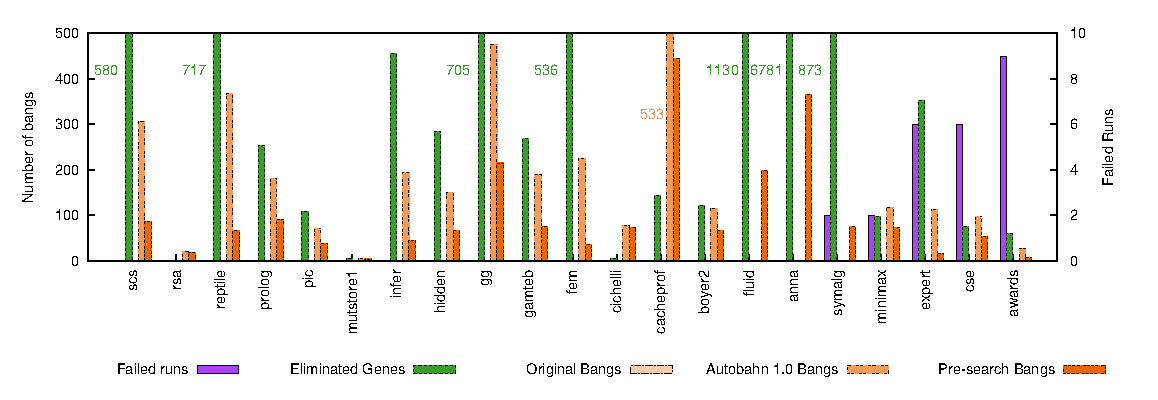
\includegraphics[width=\textwidth]{pre-aut-bangs}
\scaption{Number of bangs generated by \Ao{} vs. \Preopt{} optimizer across 21 benchmarks that had at least
one file eliminated during the \preopt{} phase. Columns that exceed
the maximum axis value are labeled with their actual values. The
benchmarks are sorted in increasing order of number of failed runs for
the \Preopt{} optimizer.}
\label{fig:preopt-bangs}
\end{figure*}

\begin{figure*}
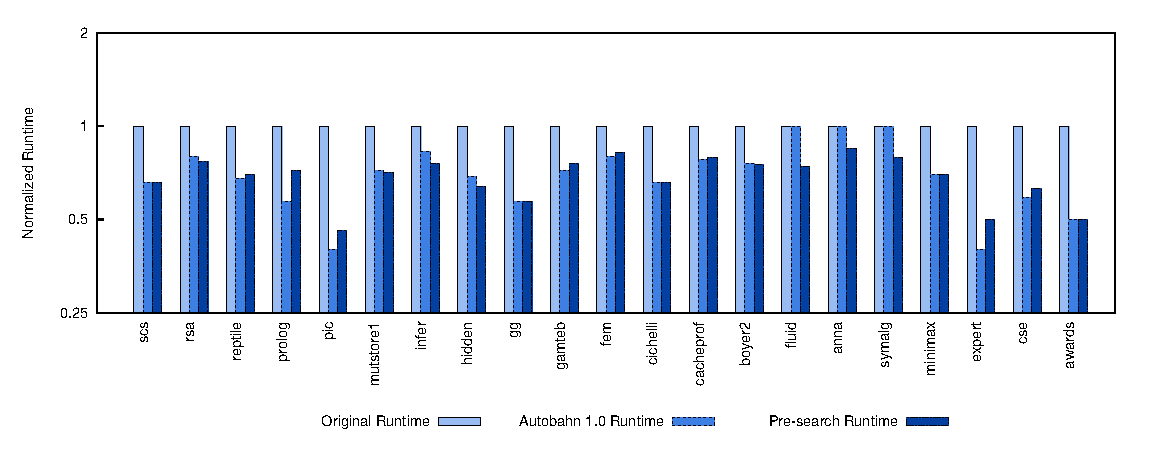
\includegraphics[width=\textwidth]{pre-aut}
\scaption{Performance runtime ratios of \Ao{} vs. \Preopt{} optimizer
across 21 benchmarks that had at least one
file eliminated during the \preopt{} phase. The x-axis
is on a base-2 log scale. The benchmarks appear in the same order as
in \figref{fig:preopt-bangs}.}
\label{fig:preopt-runtime}
\end{figure*}

%----------------------------------------------------------------------------------------
%   SECTION 3
%----------------------------------------------------------------------------------------

\section{\Preopt{} File Elimination}

\label{sec:file-elim}

The \preopt{} phase identifies 6 benchmarks among the 60 in our suite
as unsuitable for optimization when the \hotspotcost{}
threshold is set to 6\%:  \texttt{awards}, \texttt{callback001},
\texttt{callback002}, \texttt{mutstore2}, \texttt{sorting}, and \texttt{threads007}. As
expected, when attempting to
optimize \texttt{awards}, \texttt{sorting},
and \texttt{threads007}, \Ao{} consistently fails, returning
the \unimp{} runtime code. However, \Ao{} was able to
successfully optimize the other programs. Through inspection, we
concluded that \texttt{callback002} would have benefited from a
lower \hotspotcost{} threshold as its most costly hot spot takes up
3.9\% of the program runtime. Both \texttt{callback001}
and \texttt{threads007} would have benefited from inspecting heap
profiles instead of time and allocation profiles as the costs
associated with their hot spots were noticeably larger in heap
allocations while remaining insignificant in runtime
costs. The \texttt{mutstore2} program's performance fluctuated wildly
even without bangs in it. For example, its measured runtime was as low
as 60\% - 80\% of its original runtime in one-third of the experiments
we ran with no bangs in the program. Therefore, the optimization
results were likely skewed by the fluctuating runtime.

%----------------------------------------------------------------------------------------
%   SECTION 4
%----------------------------------------------------------------------------------------

\section{\Preopt{} File Addition}

To demonstrate the effectiveness of using the \preopt{} phase to
expand Autobahn's coverage for improved optimization results, we
tested our approach on the \texttt{sumList} microbenchmark. We
created \texttt{sumList} to simulate the scenario in which a
programmer references code from an external library or external file
that contains \hotspots{} but is not within the current optimization
coverage.

The \texttt{sumList} program's \texttt{Main.hs} file contains only one
function: a main function that constructs a list of integers from 1 to
1,000,000 and then calculates the sum of all integers in the list using an
external \textit{sum} function located in \texttt{Sum.hs}. Users
may decide to set the optimization coverage to [\texttt{Main.hs}],
because they are interested in making the main program run
faster. However, as demonstrated in \figref{fig:sumList}, \Ao{} was only able to
improve program performance by 3\%, even when it was able to
exhaustively search the possible bang locations in the 6 lines of code in the \texttt{main}
function. Upon inspecting the results, users may be mistaken in
believing that their program runtime cannot be improved
further.

But there are indeed other opportunities to speed up \textit{sumList}
located in places that the users did not think about. If the users were
to rerun the optimization using the \preopt{} phase, then GHC's time and
allocation profile indicates that the largest \hotspotcost{} was 9.5\%
and located in lines 7 to 8 in the \textit{sum} function
in \texttt{Sum.hs}. The \textit{sum} function is entirely lazy and did
not immediately compute the sum of each integer as it recursed through
the list. In the resulting log file, the \preopt{} phase
suggests
adding \texttt{Sum.hs} to the optimization coverage.
After expanding the coverage and re-running the optimization,
the resulting \texttt{sumList} ran at only 13\% of the original
runtime, a dramatic improvement.

Although the \texttt{sumList} example is short and synthetic, it shows
the larger potential for users to obtain much better optimization
results when running the \preopt{} phase in conjunction
with \Ao{}. Programmers often build upon each other's code and use
external functions that they may not be entirely familiar with or did
not consider optimizing. The \preopt{} phase can identify valuable
missed opportunities. Of
course, the addition of more files to optimize means that more bangs
might be generated. It is up to the user to decide if they want to add
the suggested files for better optimization results at the risk of
needing to inspect more bangs.
\newline

\begin{figure}
\centering
\begin{tabular}{p{3cm}p{3.5cm}p{4cm}p{1.5cm}}
\hline
Version   & Coverage & Normalized Runtime & No.Bangs \\
\hline
Original      & N/A   &   1  & 0   \\
\Ao{}       & [\texttt{Main.hs}]      & 0.97    &  2\\
Pre-optimization    & [\texttt{Main.hs}, \texttt{Sum.hs}]         & 0.13      & 4\\
\hline
\end{tabular}
\scaption{Results for \texttt{sumList} microbenchmark.}
\label{fig:sumList}
\end{figure}

%----------------------------------------------------------------------------------------
%   SECTION 5
%----------------------------------------------------------------------------------------

\section{\Postopt{} Bang Reduction}

To assess the effectiveness of the \postopt{} phase,
we compare the results of running \Ao{} with running
the \textit{\Postopt{} optimizer} comprised of \Ao{} followed by
the \postopt{} phase.
\cut{
Already discussed and so not necessary:
Similarly, we took the mean of running the
program ten times on the NoFib benchmark suite while optimizing on
runtime only, and set both \hotspotcost{} and \absim{} thresholds to
6\%.
A benchmark is successfully optimized if \Ao{} improved its
performance by at least 6\% after optimization. }
Figures~\ref{fig:post-bangs-all} and \ref{fig:post-ratio-all}
give the number of bangs and the runtime performance ratios,
respectively, for the 21 benchmarks that \At{} successfully optimized on all 10 runs.
Figures~\ref{fig:post-bangs-some} and \ref{fig:post-ratio-some}
give the number of bangs and the runtime performance ratios, respectively,
for the 28 benchmarks on which \At{} was partially successful,
sorted in increasing order of \At{}'s failure rate.
We do not show the results from the remaining 12 benchmarks that \At{}
failed to optimize on every run since the numbers for those benchmarks
would be unchanged from the original program.  \figref{fig:post-failures} shows how
frequently a benchmark failed at the \Ao{} stage vs. how frequently it
failed at the \postopt{} phase. The graph shows that the majority of \Postopt{} optimizer fails are
caused by failures at the \Ao{} stage, which produces a poorly
performing set of bangs for the \postopt{} phase to
minimize. Therefore, benchmarks that failed at the \Ao{} stage are
highly likely to fail during  the \postopt{} phase as well.


Figures~\ref{fig:post-bangs-all} and \ref{fig:post-bangs-some} show
that the number of bangs eliminated by the \Postopt{} optimizer is quite
significant: on average \postBangs{}. Figures~\ref{fig:post-ratio-all}
and~\ref{fig:post-ratio-some} show the corresponding runtime
performance ratios of each optimized program. In most benchmarks,
the \Postopt{} optimizer does
a little worse than \Ao{}, on average \postRatioWorse{} worse, because
the \postopt{} phase only preserves bangs that affect program
runtime by at least the \absim{} threshold (6\% in these experiments).
If users want to
maintain higher levels of optimization,
they can lower the \absim{} threshold so the minimizer becomes less
aggressive in bang elimination. That way, more bangs will be
preserved, but runtime performance will
improve.

Looking at these results in more detail,
the \texttt{callback001} and \texttt{pic} benchmarks are good
examples of when a program has no cost centers that meet
the \hotspotcost{} threshold, so the \postopt{} phase eliminated all their bangs.
In these cases, a lower threshold would have
helped discover useful bangs that are located in the relatively colder locations.
The data for \texttt{anna} and \texttt{fluid}
show that while \Ao{} found bangs that triggered a \nonterm{} runtime
code, \postopt{} bang elimination was able to eliminate
the \dangerous{} bangs that caused the bad behavior and instead produce
successful optimization results.

\begin{figure*}
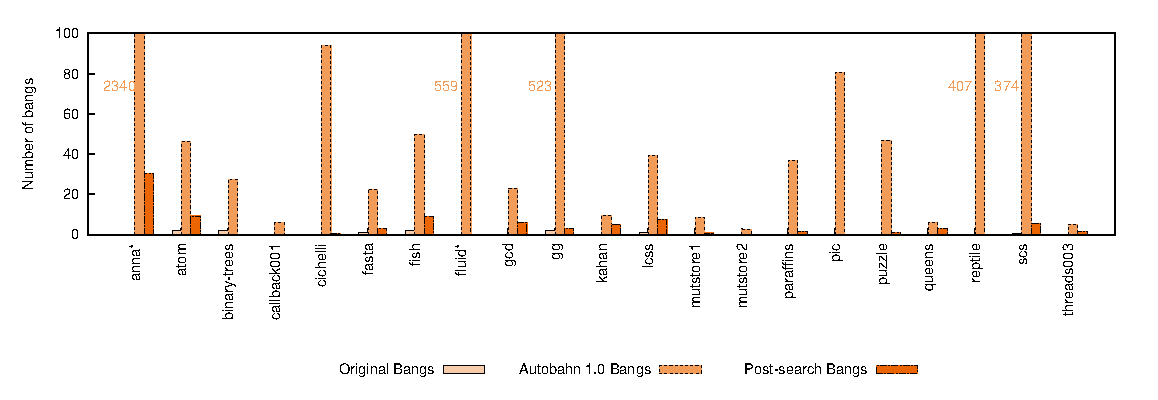
\includegraphics[width=\textwidth]{aut-post-bangs}
\scaption{Number of bangs generated by \Ao{} vs. \Postopt{} optimizer
across 21 benchmarks that \At{} successfully optimized
every time. Columns that exceed the maximum axis value are labeled
with their actual values. }
\label{fig:post-bangs-all}
\end{figure*}

\begin{figure*}
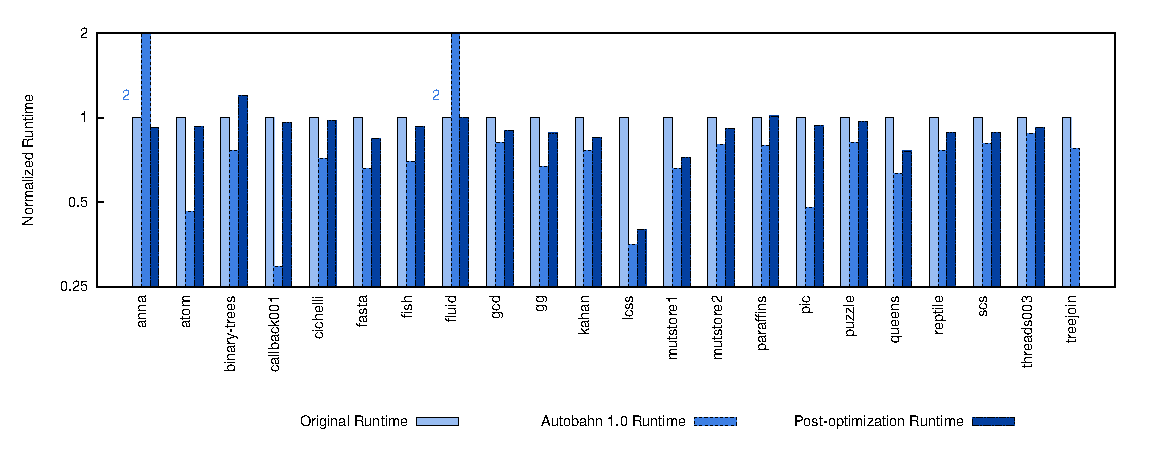
\includegraphics[width=\textwidth]{aut-post}
\scaption{Performance runtime ratios of \Ao{} vs. \Postopt{} optimizer
across 21 benchmarks that \At{} successfully
optimized every time. The x-axis is on a base-2 log scale.
For the *-ed benchmarks, \Ao{} generated non-terminating
optimization results, but the \postopt{} phase removed
the \dangerous{} bangs and succeeded in optimizing the program. }
\label{fig:post-ratio-all}
\end{figure*}

\begin{figure*}
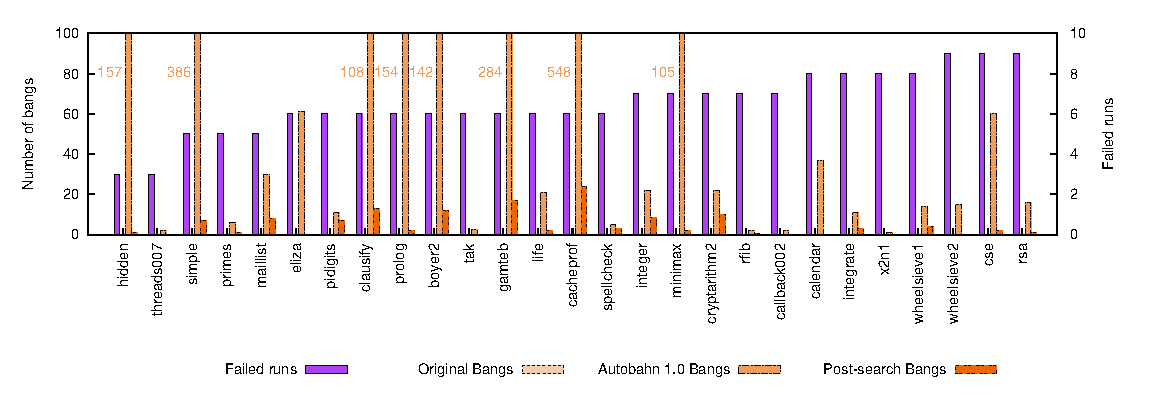
\includegraphics[width=\textwidth]{ap-partial-bangs}
\scaption{Number of bangs generated by \Ao{} vs. \Postopt{} optimizer
across 27 benchmarks that \At{} successfully optimized on some runs. Failure rate
out of 10 runs is shown. Columns that exceed
the maximum axis value are labeled with their actual values.
The benchmarks are sorted in increasing order of \At{} failure rate. }
\label{fig:post-bangs-some}
\end{figure*}

\begin{figure*}
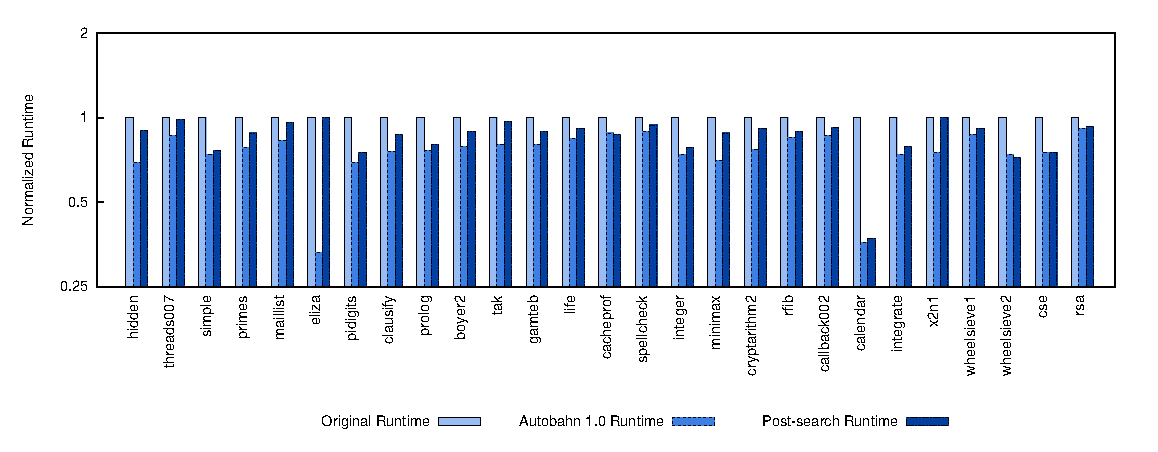
\includegraphics[width=\textwidth]{ap-partial}
\scaption{Performance runtime ratios of \Ao{} vs. \Postopt{} optimizer
across 27 benchmarks that \At{} successfully optimized on some runs.
The x-axis is on a base-2 log scale.
}
\label{fig:post-ratio-some}
\end{figure*}

\begin{figure*}
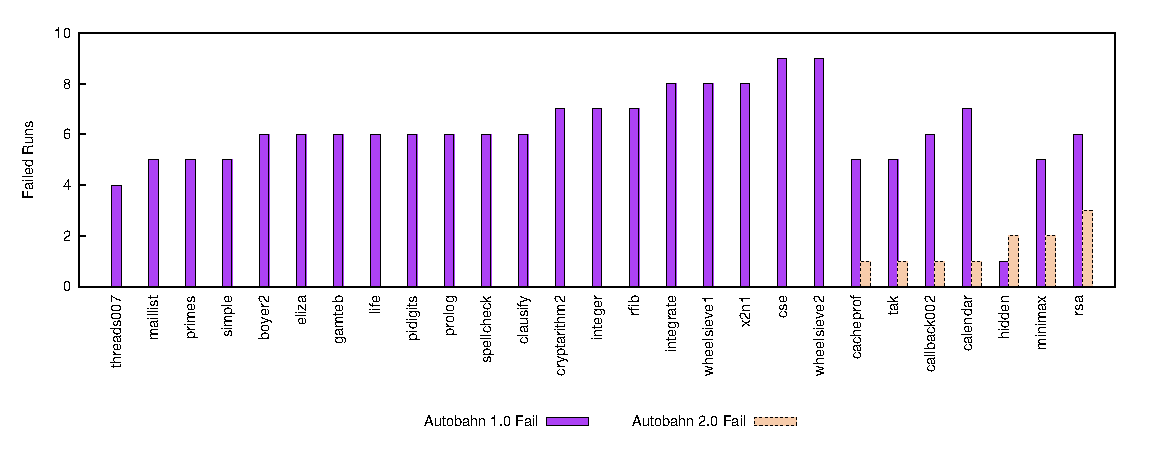
\includegraphics[width=\textwidth]{aut-post-fail}
\scaption{Frequency of failures attributable to \Ao{} vs
the \postopt{} phase across 27
benchmarks on which optimization sometimes succeeded. Benchmarks are sorted in
increasing order of \Postopt{} optimizer failure rate. }
\label{fig:post-failures}
\end{figure*}

%----------------------------------------------------------------------------------------
%   SECTION 6 
%----------------------------------------------------------------------------------------

\section{\At{}: Combining \preopt{} and \postopt{}}

To evaluate the overall effectiveness of \At{}, we ran the complete
tool chain on our NoFib benchmarks 10 times. Figures~\ref{fig:2-bangs-26}, \ref{fig:2-ratio-26}, \ref{fig:2-bangs-52},
and \ref{fig:2-ratio-52} presents the numbers of recommended bangs and
the runtime performance ratios on the 52 benchmarks that \At{}
successfully optimized at least once using runtime as the \profm{}.
All benchmarks are sorted in increasing order of \At{} failure rate.

Out of those 60 programs, the \preopt{} phase eliminated 5 because they had no \hotspots{}.  
On another 3 benchmarks, neither \Ao{} nor \At{}
successfully found an optimization on any run.
It is interesting to note that only these 8
benchmarks consistently failed under \At{}, while 12
consistently failed under the \Postopt{} optimizer.
This observation shows that the \preopt{} phase successfully
increased the effectiveness of the later optimization phases.

Overall, \At{} reduced the number of bangs generated by 90.2\%
with an optimization degradation of 15.7\%.
We split the data into two graphs of 26 benchmarks each for bang counts
(Figures~\ref{fig:2-bangs-26} and~\ref{fig:2-bangs-52})
and for runtime performance ratios
(Figures~\ref{fig:2-ratio-26} and~\ref{fig:2-ratio-52})
for legibility.
Finally, \figref{fig:2-failures} shows how frequently a benchmark
failed at the \Ao{} stage versus at the end of \At{}. As with
the \postopt{} optimizer, the majority of runs failed at the \Ao{} stage.


While most benchmarks consistently showed significant bang reduction
with minimal optimization degradation under \At{}, a few benchmarks stand
out. The \texttt{expert} and \texttt{calendar} benchmark not only had
bangs reduced by 79.41\% and 97.63\% respectively, but also
experienced performance \textit{improvements} of 27.60\% and 14.82\%
respectively. It is worth noting that both benchmarks failed
more times than they succeeded, so such results are not guaranteed to
be replicable in every run. The \texttt{atom} benchmark is also noteworthy
because the \postopt{} phase eliminated all bangs
generated by \Ao{}, yet it still had a runtime performance ratio of
0.78. This finding suggests that \texttt{atom}'s original
runtime fluctuates by a significant amount on its own. It also
suggests that \texttt{atom}'s overall performance
improvement is achieved through the accumulation of speedups at many
relatively cold cost centers, so lowering \At{}'s \hotspotcost{}
might result in a better performance improvement.

\begin{figure*}
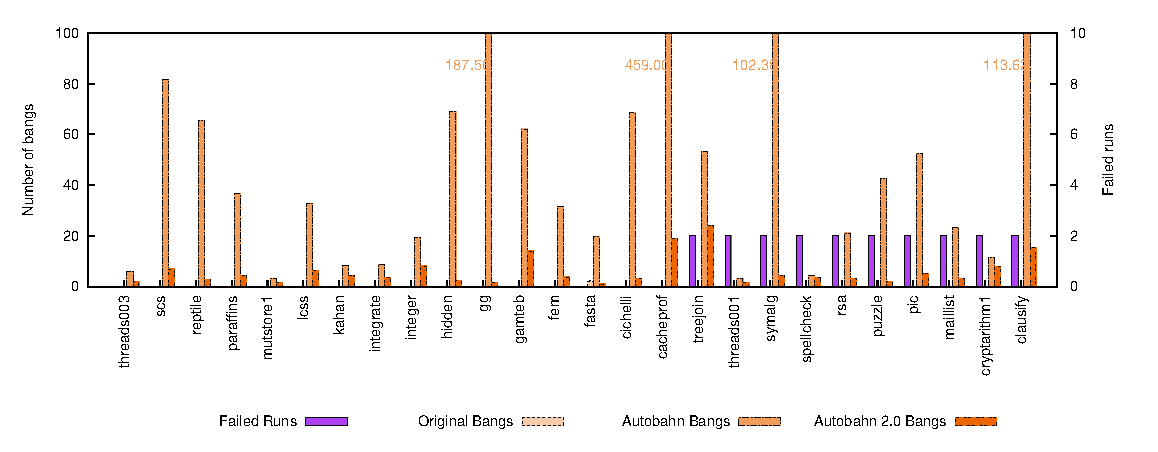
\includegraphics[width=\textwidth]{pap0-bangs}
\scaption{Number of bangs generated by \Ao{} vs. \At{} across the first
26 of 52 benchmarks that \At{} successfully optimized
at least once using runtime as the \profm{}. Failure
rate out of 10 runs is shown. Benchmarks are sorted in increasing order of
failure rate. Columns that exceed the maximum axis value are labeled
with their actual values.}
\label{fig:2-bangs-26}
\end{figure*}

\begin{figure*}
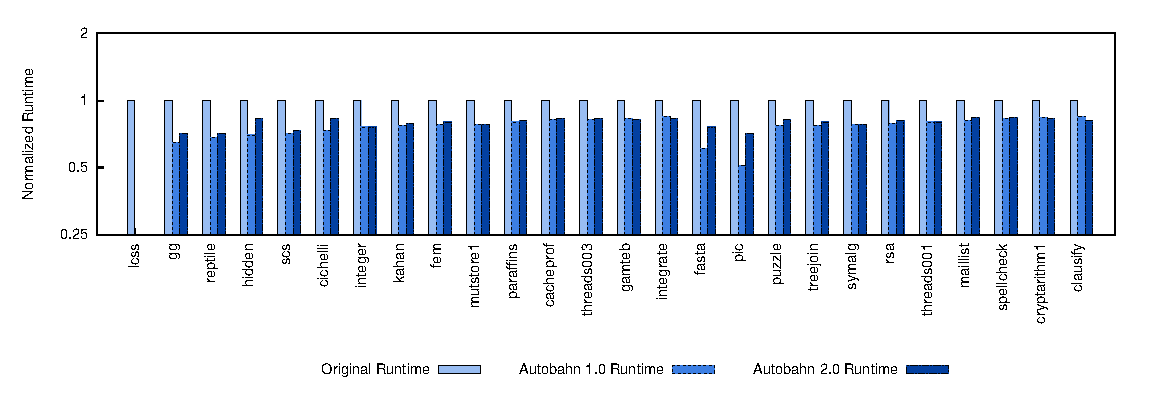
\includegraphics[width=\textwidth]{pap0}
\scaption{Runtime performance ratios of \Ao{} vs. \At{} across
the first 26 of 52 benchmarks that \At{} successfully optimized at least
once using runtime as the \profm{}. The x-axis is on a base-2 log scale.}
\label{fig:2-ratio-26}
\end{figure*}

\begin{figure*}
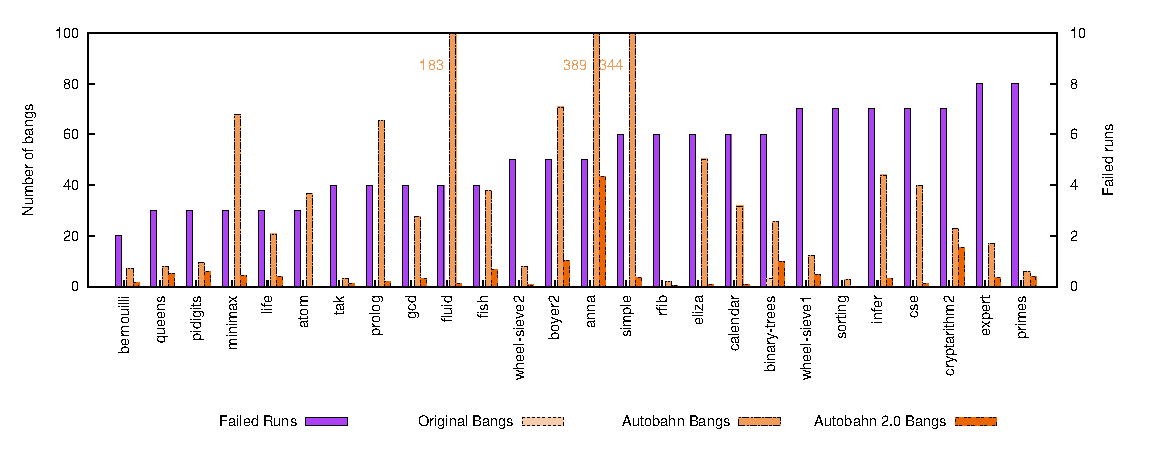
\includegraphics[width=\textwidth]{pap1-bangs}
\scaption{Number of bangs generated by \Ao{} vs. \At{} across the
remaining 26 of 52 benchmarks that \At{} successfully optimized at least
once using runtime as the \profm{}. Failure rate out of 10 runs is shown. 
Benchmarks are sorted in
increasing order of failure rate. Columns that exceed the maximum axis
value are labeled with their actual values. }
\label{fig:2-bangs-52}
\end{figure*}

\begin{figure*}
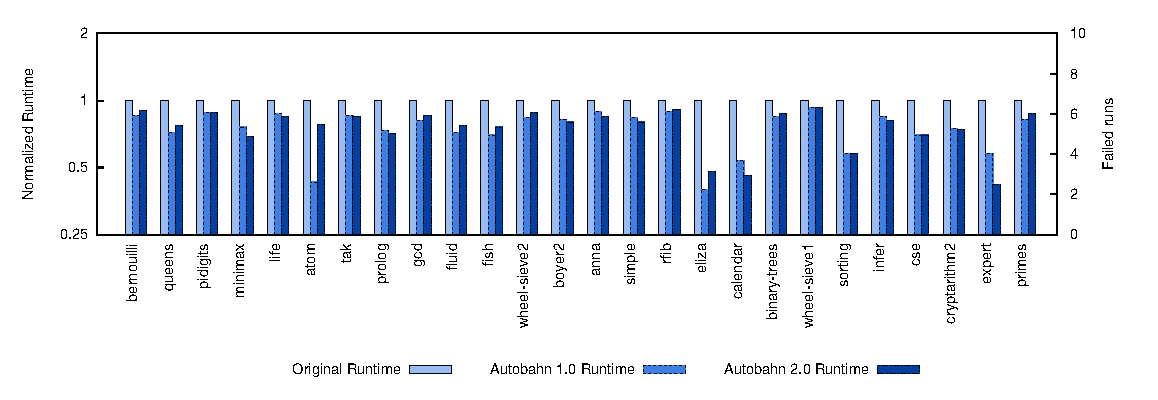
\includegraphics[width=\textwidth]{pap1}
\scaption{Runtime performance ratios of \Ao{} vs. \At{} across the
remaining 26 of 52 benchmarks that \At{} successfully optimized at least
once using runtime as the \profm{}. The x-axis is on a base-2 log scale.
}
\label{fig:2-ratio-52}
\end{figure*}

\begin{figure*}
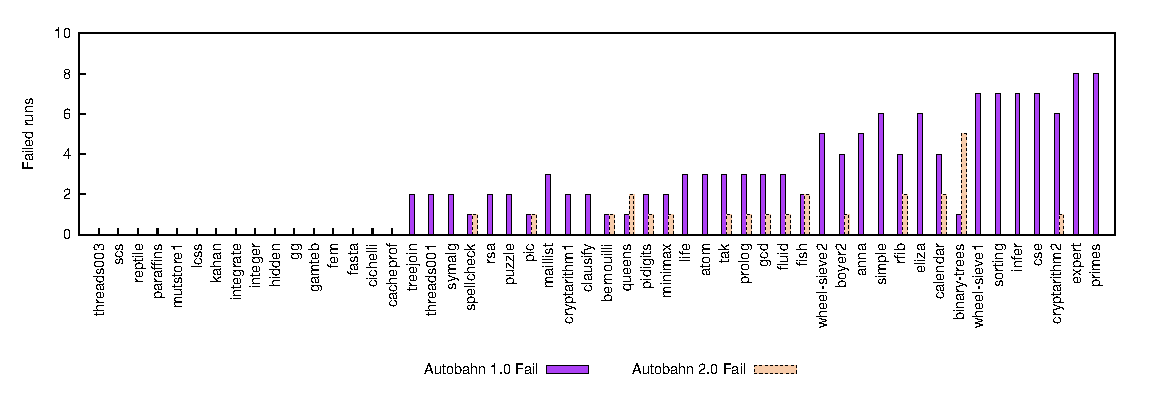
\includegraphics[width=\textwidth]{pap-fail}
\scaption{Frequency of failure attributable to \Ao{} versus \At{} across the 36
benchmarks that \At{} sometimes successfully optimized using runtime as the \profm{}. 
Benchmarks are sorted in increasing order of \At{} failure rate. }
\label{fig:2-failures}
\end{figure*}

\subsection{Runtime vs. memory allocations as \profm{}}

To evaluate whether there is a measurable performance difference in using 
memory allocations over runtime as the \profm{}, we also ran \At{} on the 
60 benchmarks 10 times (NOTE: will change this to 10 times when I finish running
all of them) using memory allocations as the \profm{}. 
Figures~\ref{fig:2-bangs-26-HA}, \ref{fig:2-ratio-26-HA}, \ref{fig:2-bangs-52-HA},
and \ref{fig:2-ratio-52-HA} presents the numbers of recommended bangs and
the runtime performance ratios on the 27 benchmarks that \At{}
successfully optimized at least once using memory allocations as the \profm{}.

\begin{figure*}
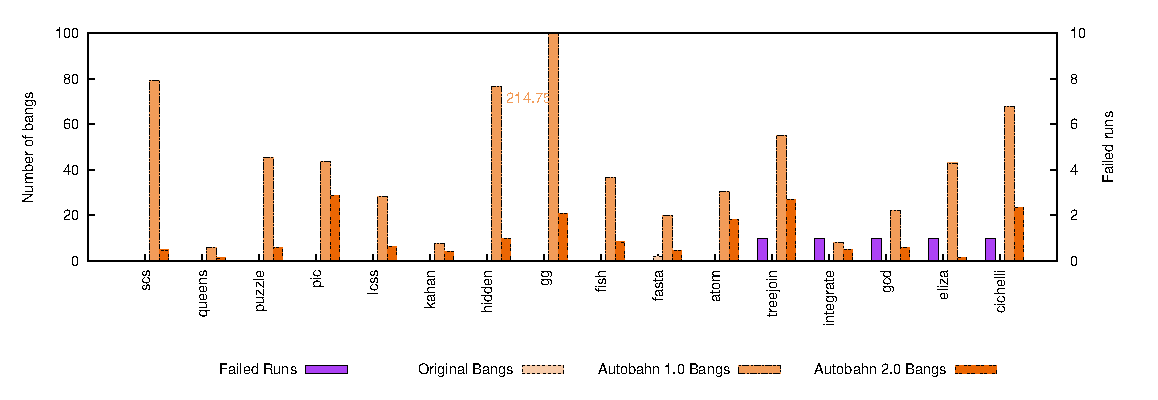
\includegraphics[width=\textwidth]{HA-bpapA}
\scaption{Number of bangs generated by \Ao{} vs. \At{} across the first
16 of 32 benchmarks that \At{} successfully optimized
at least once using memory allocations as the \profm{}. Failure
rate out of 10 runs is shown. Benchmarks are sorted in increasing order of
failure rate. Columns that exceed the maximum axis value are labeled
with their actual values.}
\label{fig:2-bangs-26-HA}
\end{figure*}

\begin{figure*}
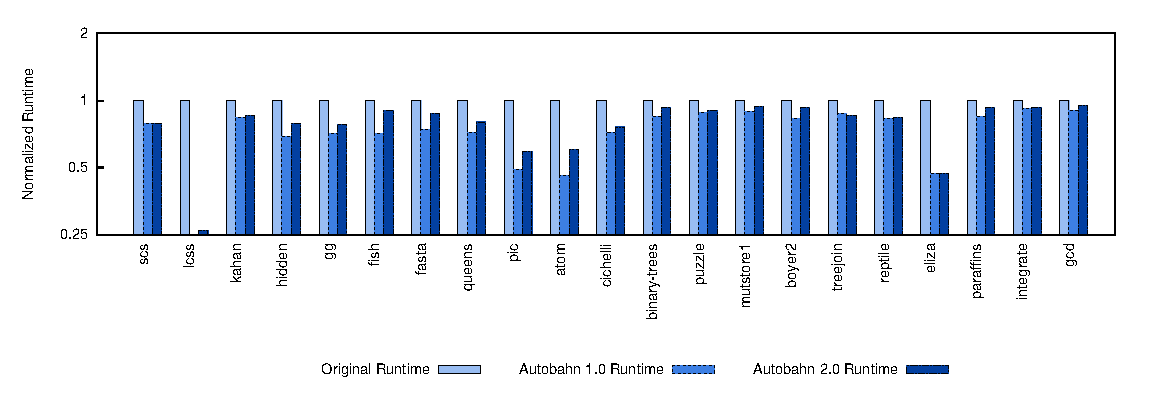
\includegraphics[width=\textwidth]{HA-papA}
\scaption{Runtime performance ratios of \Ao{} vs. \At{} across
the first 16 of 32 benchmarks that \At{} successfully optimized at least
once using memory allocations as the \profm{}. The x-axis is on a base-2 log scale.}
\label{fig:2-ratio-26-HA}
\end{figure*}

\begin{figure*}
\includegraphics[width=\textwidth]{HA-bpapb}
\scaption{Number of bangs generated by \Ao{} vs. \At{} across the remaining 
15 of 32 benchmarks that \At{} successfully optimized
at least once using memory allocations as the \profm{}. Failure
rate out of 10 runs is shown. Benchmarks are sorted in increasing order of
failure rate. Columns that exceed the maximum axis value are labeled
with their actual values.}
\label{fig:2-bangs-52-HA}
\end{figure*}

\begin{figure*}
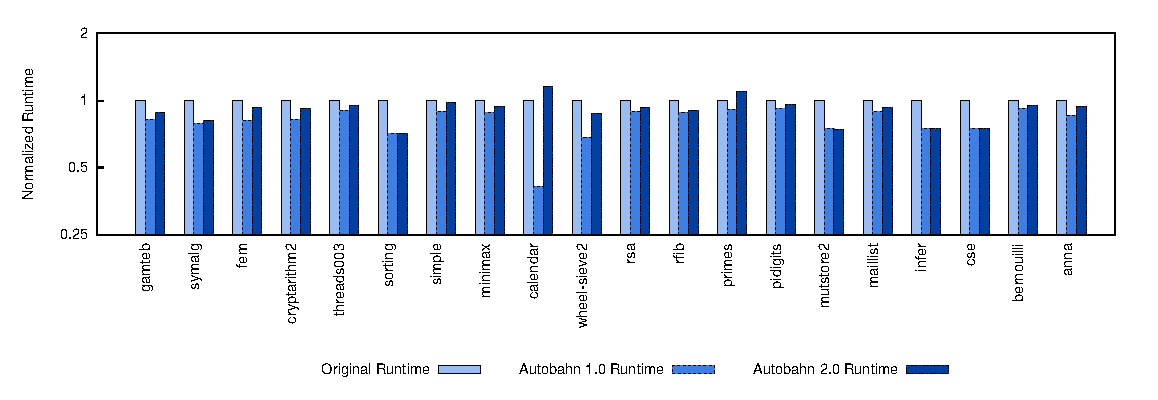
\includegraphics[width=\textwidth]{HA-papB}
\scaption{Runtime performance ratios of \Ao{} vs. \At{} across
the remaining 15 of 32 benchmarks that \At{} successfully optimized at least
once using memory allocations as the \profm{}. The x-axis is on a base-2 log scale.}
\label{fig:2-ratio-52-HA}
\end{figure*}


\begin{figure*}
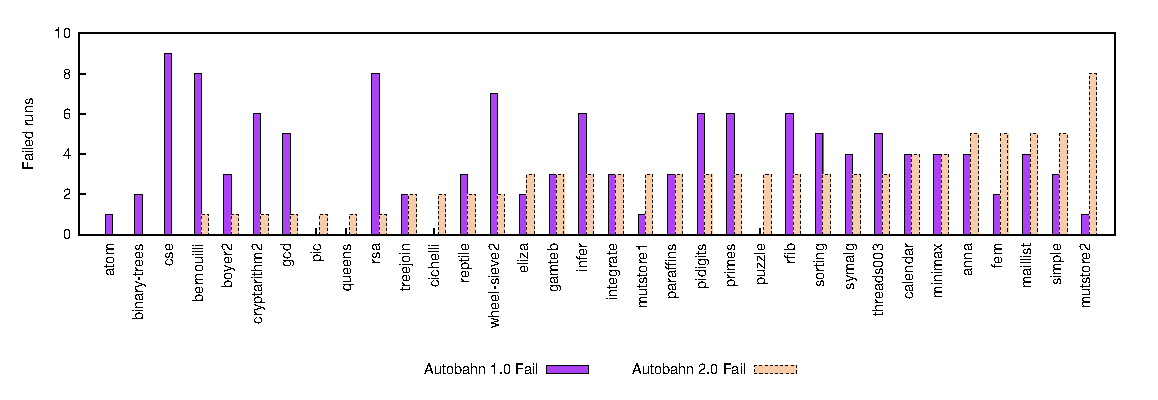
\includegraphics[width=\textwidth]{HA-pap-fail}
\scaption{Frequency of failure attributable to \Ao{} versus \At{} across the 45 
benchmarks that \At{} sometimes successfully optimized using memory allocations as the \profm{}. 
Benchmarks are sorted in increasing order of \At{} failure rate. }
\label{fig:failures-HA}
\end{figure*}

\begin{figure*}
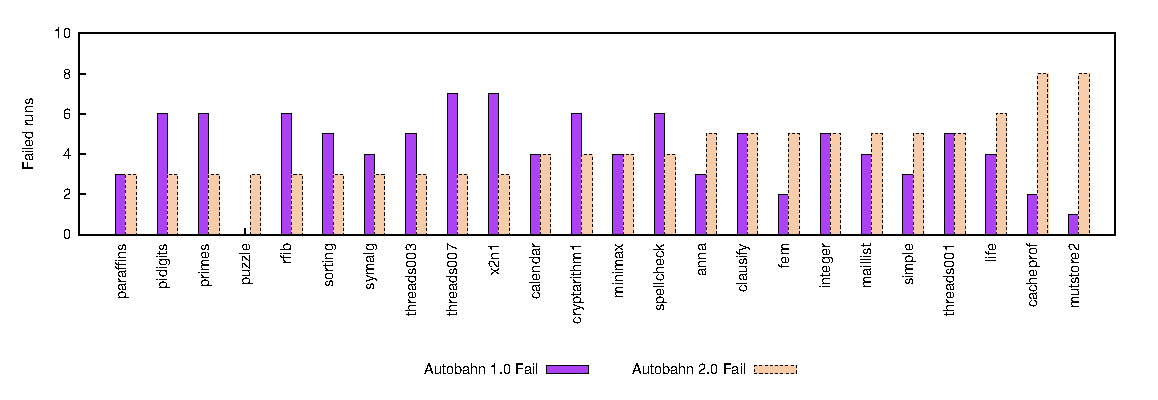
\includegraphics[width=\textwidth]{HA-pap-fail-2}
\scaption{Frequency of failure attributable to \Ao{} versus \At{} across the 45
benchmarks that \At{} sometimes successfully optimized using memory allocations as the \profm{}.
Benchmarks are sorted in increasing order of \At{} failure rate. }
\label{fig:2-failures-HA}
\end{figure*}

%----------------------------------------------------------------------------------------
%   SECTION 7
%----------------------------------------------------------------------------------------

\section{Case Study: \At{} On \texttt{gcSimulator}}
As a case study, we ran \At{} on \texttt{gcSimulator}, which is a
garbage collection simulator that consumes program execution traces
produced by the Elephant Tracks~\cite{Ricci13} monitoring system.  The
simulator comprises 2026~lines of code spread across 20~source code
files. To keep \Ao{} runtime within reasonable ranges, we used the
first 1M of the \texttt{batik} trace file from the DaCapo
benchmarks~\cite{Blackburn06} as the representative input.  For this
case study, we lowered the \absim{} threshold to 1\%
because \texttt{gcSimulator} does not have many \hotspots{} at higher
thresholds.  Once \At{} was done optimizing, we evaluated the
resulting program on larger trace file sizes of 100M and 500M. Because
running the simulator on the full 6184M trace size took too
long with or without optimization, we did not record results for the
full trace.

\Ao{} produces results that run
faster on representative input as well as on larger trace files.
\At{} was able to generate similar performance results with many fewer
bangs (125 vs. 690), as demonstrated in \figref{tab:gc}. 
While \figref{tab:gc} presents results from running \At{} using runtime
as the profiling metric, we also ran the same experiment using heap
allocations as the profiling metric. We did not find a significant
difference in using either profiling metric.

\begin{table}
\centering

\begin{tabular}{p{3cm}p{3cm}p{5cm}p{1.5cm}}
%\begin{tabular}{lllr}
\hline
Version   & File Size (M) & Runtime Performance Ratio& No.Bangs \\
\hline
Original      & 1       & 1         & 0   \\
              & 100     & 1         & 0 \\
              & 500     & 1         & 0 \\
\Ao{}         & 1       & 0.45      &  690\\
              & 100     & 0.33      &  690\\
              & 500     & 0.32      & 690\\
\At{}         & 1       &  0.58     & 125    \\
              & 100     & 0.37      & 125      \\
              & 500     & 0.38      & 125    \\

\hline
\end{tabular}
\scaption{Performance results for \texttt{gcSimulator}.}
\label{tab:gc}
\end{table}
 
\chapter{Related Work and Future Work} 

\label{Chapter6} % \ref{ChapterX}

%----------------------------------------------------------------------------------------
%	SECTION 1
%----------------------------------------------------------------------------------------

\section{\Ao{} and Other Methods of Managing Laziness}

The current strictness analyzer in GHC uses backward abstract
interpretation to identify locations that can be eagerly
evaluated~\cite{Sergey14}. The analysis is sound but necessarily
approximate because it is static and the underlying property is
undecidable. The analysis only marks locations as strict if it can
guarantee termination on all possible inputs, not just realistic ones,
since it is part of the compiler.  Like \Ao{}, \At{} leverages the
advantages of being dynamic and not attempting to guarantee
termination on all inputs.  Instead, \Ao{} allows users to decide if
the annotations are safe on the intended inputs.

Other approaches for reducing laziness include Strict
Haskell~\cite{strict-haskell}, which allows users to make entire modules strict rather than
lazy by default using the \texttt{-XStrict} and \texttt{-XStrictData} language
pragmas. Chang and Felleisen~\cite{Chang14} take the opposite
approach: they start with a program written in a strict
language and inserts laziness annotations using dynamic
profiling. It would be interesting to see if Chang and Felleisen's
method could be applied to introduce laziness to Strict Haskell
programs.

%----------------------------------------------------------------------------------------
%	SECTION 2
%----------------------------------------------------------------------------------------

\section{\At{} Improvements}

For future developments, it would be worth exploring methods to 
automatically predict which profiling metric would produce better
results so the user does not need to decide.
Similarly, we could implement thresholds
that automatically adjust themselves based on profiling results. Our
experiments show that the ideal values for \hotspotcost{} and \absim{}
thresholds vary by program to program. Adopting more flexible
thresholds that automatically adjust themselves after inspecting the
profile in the \preopt{} phase might yield better results than using
set values or asking users to provide them.


\chapter{Conclusion} 

\label{Chapter7} % \ref{ChapterX}

%----------------------------------------------------------------------------------------
%	SECTION 1
%----------------------------------------------------------------------------------------

\section{Conclusion}

Laziness is a double-edged sword: While it provides many benefits,
excessive laziness can cause poor performance. Strictness annotations
allow programmers to force eager evaluation, but its use is limited to
experienced programmers with high levels of expertise. \Ao{} uses a
genetic algorithm to automatically infer annotations to improve
program performance, but it often suggests too many bangs for users to
inspect. We have built \At{}, which uses GHC profiling feedback to
focus the search space and eliminates \useless{} bangs in a
post-processing phase.  Experiments show
that \At{} removes 90.2\% of bangs that \Ao{} recommended with only a
15.7\% optimization degradation on the NoFib benchmark,
and 81.8\% of the bangs with the same 15.7\% optimization degradation
on the \texttt{gcSimulator} case study.


%----------------------------------------------------------------------------------------
%	THESIS CONTENT - APPENDICES
%----------------------------------------------------------------------------------------

\appendix % Cue to tell LaTeX that the following "chapters" are Appendices

% Include the appendices of the thesis as separate files from the Appendices folder
% Uncomment the lines as you write the Appendices

%% Appendix A

\chapter{Frequently Asked Questions} % Main appendix title

\label{AppendixA} % For referencing this appendix elsewhere, use \ref{AppendixA}

\section{How do I change the colors of links?}

The color of links can be changed to your liking using:

{\small\verb!\hypersetup{urlcolor=red}!}, or

{\small\verb!\hypersetup{citecolor=green}!}, or

{\small\verb!\hypersetup{allcolor=blue}!}.

\noindent If you want to completely hide the links, you can use:

{\small\verb!\hypersetup{allcolors=.}!}, or even better: 

{\small\verb!\hypersetup{hidelinks}!}.

\noindent If you want to have obvious links in the PDF but not the printed text, use:

{\small\verb!\hypersetup{colorlinks=false}!}.

%\include{Appendices/AppendixB}
%\include{Appendices/AppendixC}

%----------------------------------------------------------------------------------------
%	BIBLIOGRAPHY
%----------------------------------------------------------------------------------------

\printbibliography[heading=bibintoc]

%----------------------------------------------------------------------------------------

\end{document}  
